\documentclass{article}

% Language setting
% Replace `english' with e.g. `spanish' to change the document language
\usepackage[english]{babel}

% Set page size and margins
% Replace `letterpaper' with `a4paper' for UK/EU standard size
\usepackage[letterpaper,top=2cm,bottom=2cm,left=3cm,right=3cm,marginparwidth=1.75cm]{geometry}

% Useful packages
\usepackage{amsmath}
\usepackage{graphicx}
\usepackage[colorlinks=true, allcolors=blue]{hyperref}
\usepackage{float}

\title{CS460: Assignment 2}
\author{Arya Shetty || Damon Lin}
\begin{document}
\maketitle

\section{Generating Environments}

Important note, to run on the iLab computers just use the python environment: \\
\$ source /common/system/venv/python310/bin/activate \\
The rest of the libraries were just numpy and matplotlib.
\\

Through the implementation of the functions \texttt{generate\_environment()}, \texttt{scene\_to\_file()}, \\ \texttt{scene\_from\_file()}, and \texttt{visualize\_scene()}, we represented the environment as a list of tuples containing the attributes of the obstacles.

\subsection{\texttt{generate\_environment()}}
The function \texttt{generate\_environment()} encompasses several sub-functions that assist in the task of generating an environment. These sub-functions include: \texttt{generate\_obstacle()}, \texttt{getCorners()}, \texttt{getProjection()}, and \texttt{checkCollision()}. The method will generate $n$ number of obstacles through a for loop, which then checks to see if there is a collision with anything else in the environment. If there is no collision, the function will add the generated obstacle to the environment. The \\ \texttt{checkCollision(obstacle, env)} function takes any obstacle and the environment to check for any collision. \texttt{checkCollision()} employs \texttt{getCorners()} and \texttt{getProjection} to get the edges of the obstacle to check and all other obstacles in the environment. The projection is calculated through these edges to employ the SAT (Separating Axis Theorem) to check for collisions.

\subsection{\texttt{scene\_to\_file()}}

Like any file writer, the function \texttt{scene\_to\_file(env, filename)} writes the contents in the $env$ list into the designated file. Each tuple contained in $env$ is allocated a line within the text file.

\subsection{\texttt{scene\_from\_file()}}

Similarly, the function \texttt{scene\_from\_file(filename)} retrieves the contents within the specified file and appends them to a new $env$ list. However, storing the tuples within the text file contains parentheses and commas to delineate the tuples from one another. Thus, we strip each line of the parentheses and group the values separated by commas as tuples to append to $env$.

\subsection{\texttt{visualize\_scene()}}

After initializing a figure to plot the environment onto, iterate through the environment list $env$ to get all the obstacles and their properties. For each obstacle, perform an affine transformation using the \texttt{Affine2D} method to visualize an object and its orientation properly. Finally, add these obstacles as rectangles to the figure and show the plot.

\begin{figure} [H]
    \centering
    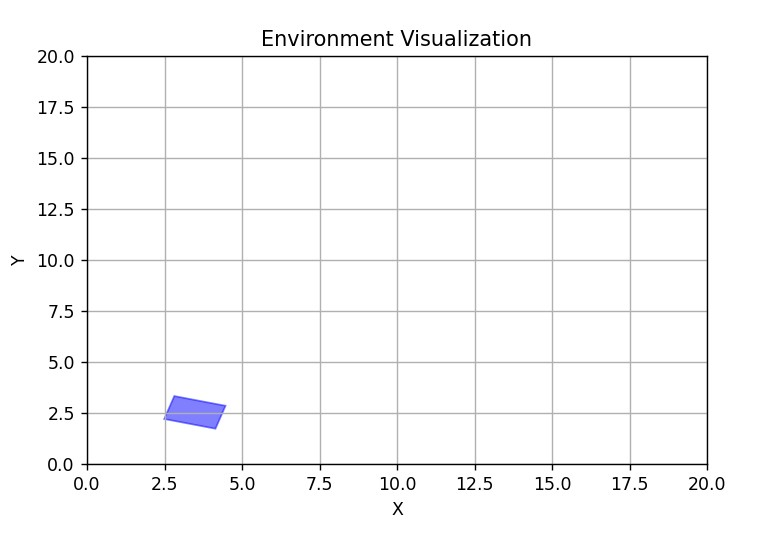
\includegraphics[width=0.7\linewidth]{latex_media/env1.jpg}
    \caption{Environment 1: 1 obstacle}
\end{figure}

\begin{figure} [H]
    \centering
    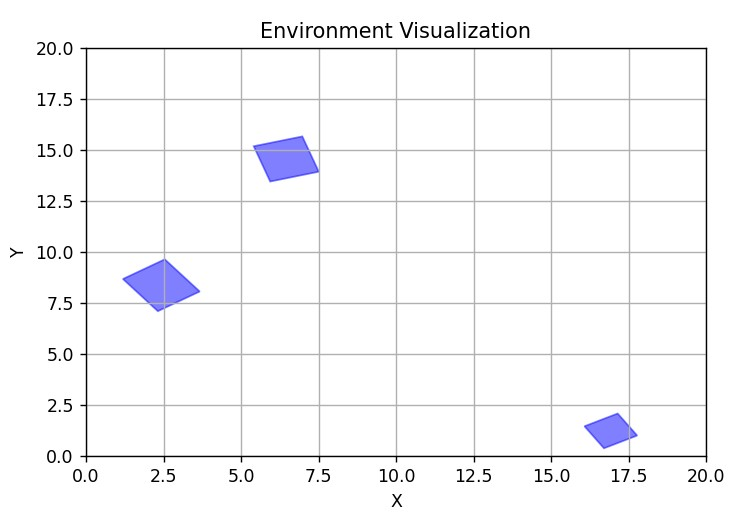
\includegraphics[width=0.7\linewidth]{latex_media/env2.jpg}
    \caption{Environment 2: 3 obstacles}
\end{figure}

\begin{figure} [H]
    \centering
    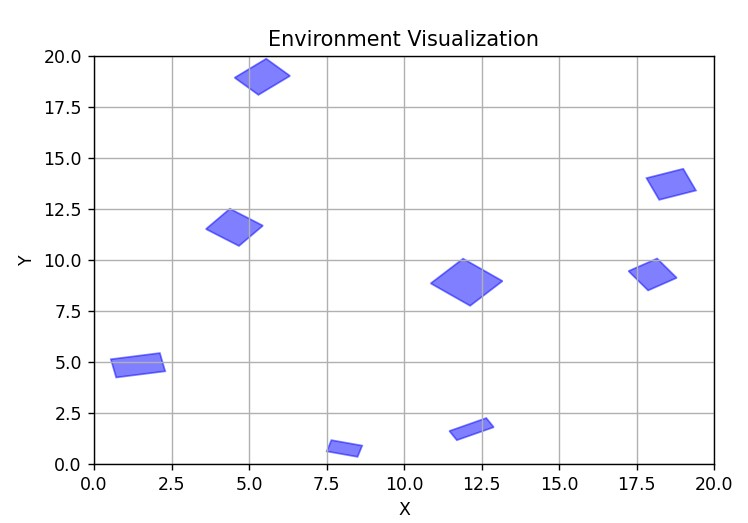
\includegraphics[width=0.7\linewidth]{latex_media/env3.jpg}
    \caption{Environment 3: 8 obstacles}
\end{figure}

\begin{figure} [H]
    \centering
    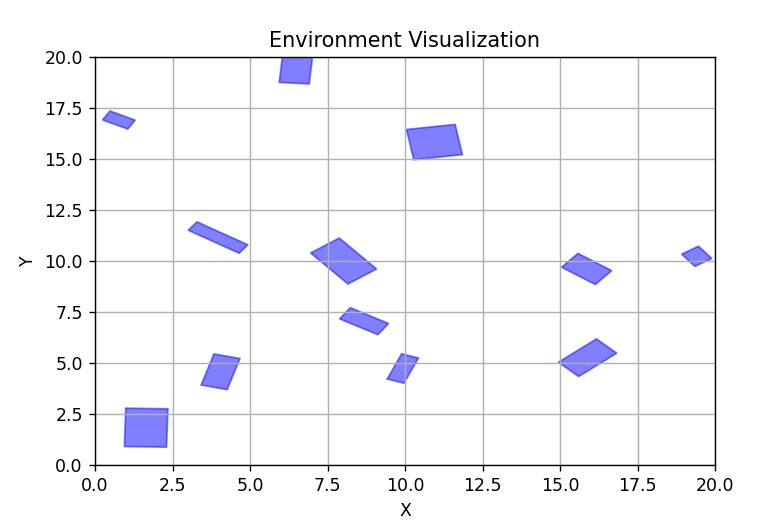
\includegraphics[width=0.7\linewidth]{latex_media/env4.jpg}
    \caption{Environment 4: 12 obstacles}
\end{figure}

\begin{figure} [H]
    \centering
    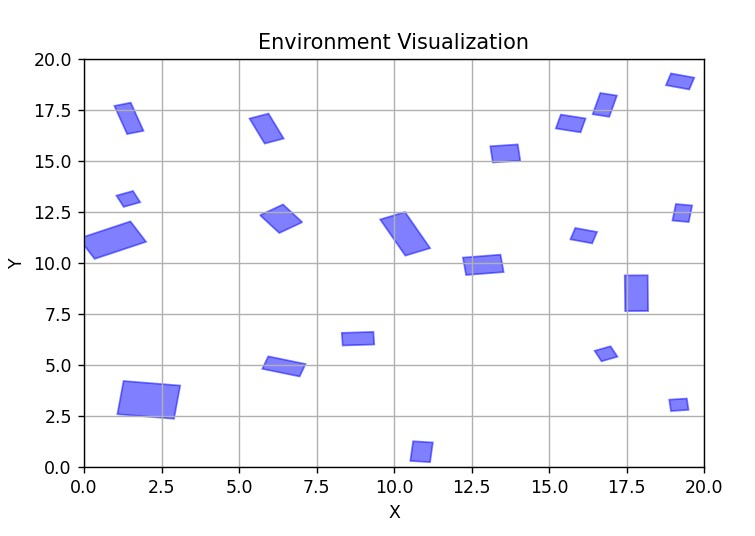
\includegraphics[width=0.7\linewidth]{latex_media/env5.jpg}
    \caption{Environment 5: 20 obstacles}
\end{figure}

\section{Nearest Neighbors with Linear Search Approach}

We implemented the nearest neighbors by first getting all the configurations from a file. Then, for each configuration, we had a distance calculation for "freeBody" using Euclidean distance for the (x, y) position and then angular distance for the (theta) and took the sum of those two. We accounted for angle wrapping by taking the difference and adding pi to make the range [0,2$\pi$], then use modulo operation of 2$\pi$ to keep it in the range, finally, we subtracted $\pi$ to bring it back. When taking the sum, we also weigh the orientation to have half the importance of position since it is more of a priority. Then we sort the configurations by distance. For the arm robots, we compared the joint angles. We use the same angular distance method and ensure the angle wrapping is handled; then, we take the square root of the sum between the two angular distances squared for the distance. The topology for the arm robot is a torus, as each link would be a circle $S_1 x S_1$. The topology for the free body would be a 2D plane and then a circle for orientation, so $R^2 x S^1$. Below are images for the free body and arm showing the nearest neighbor configurations and the query point, which is the target configuration (If you want to see the list of configurations used, it's in the code; the one for the free body is configs1.txt and for arm it's configs2arm.txt). (Additionally, this code is run by "python nearest\_neighbors.py" and to define what robot, target, k, and file to use you can edit the main function in the code)

\begin{figure} [H]
    \centering
    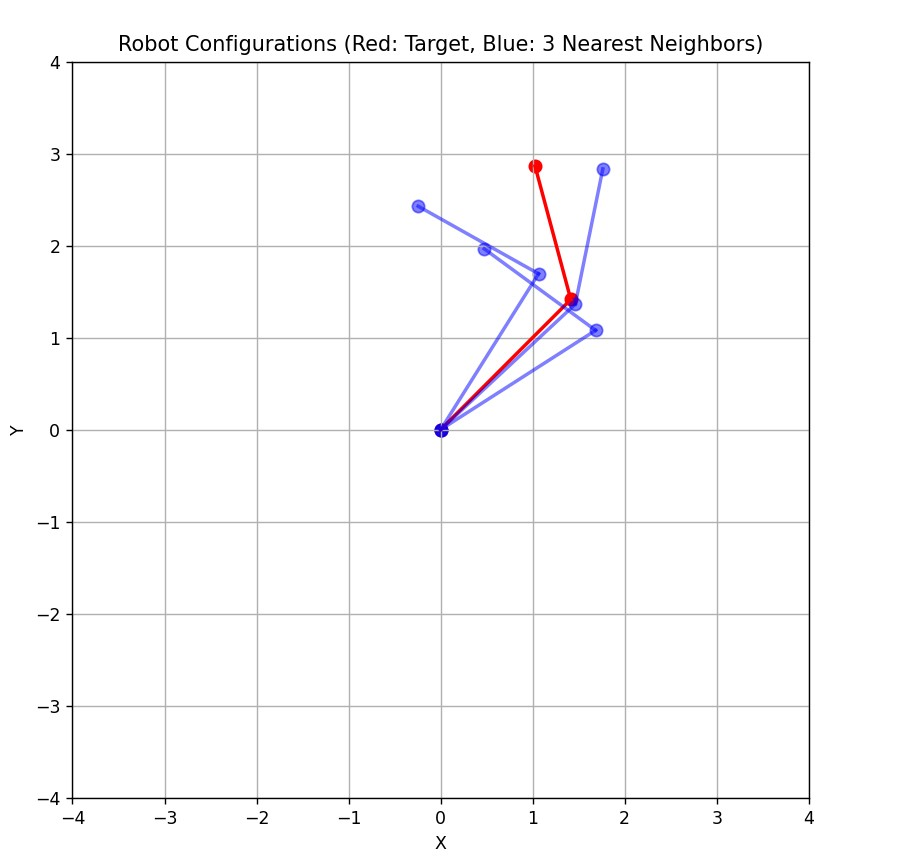
\includegraphics[width=0.5\linewidth]{latex_media/nearestArm1.jpg}
    \caption{Query: (0.79, 1.04)
    Nearest configurations: [(0.75, 0.62), (1.01, 1.62), (0.57, 1.94)]}
\end{figure}

\begin{figure} [H]
    \centering
    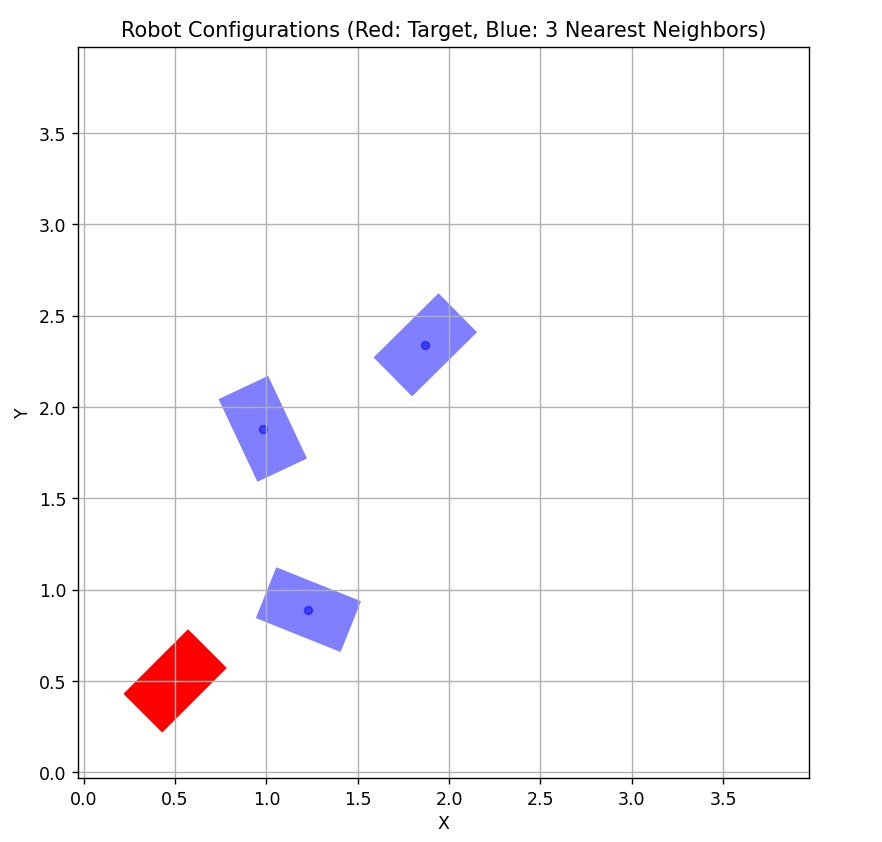
\includegraphics[width=0.5\linewidth]{latex_media/nearestFreeBody1.jpg}
    \caption{Query: (0.5, 0.5, 0.79)
    Nearest configurations: [(1.23, 0.89, 2.76), (0.98, 1.88, 2.01), (1.87, 2.34, 0.78)]
    }
\end{figure}

\begin{figure} [H]
    \centering
    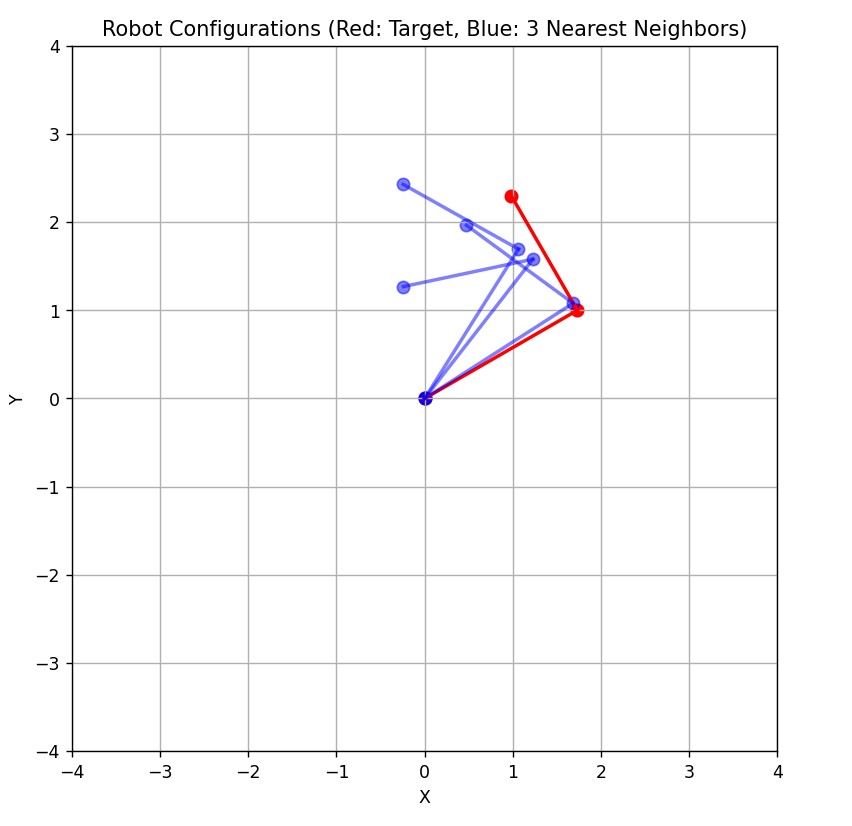
\includegraphics[width=0.5\linewidth]{latex_media/nearestArm2.jpg}
    \caption{Query: (0.52, 1.57)
    Nearest configurations: [(0.57, 1.94), (1.01, 1.62), (0.91, 2.44)]}
\end{figure}

\begin{figure} [H]
    \centering
    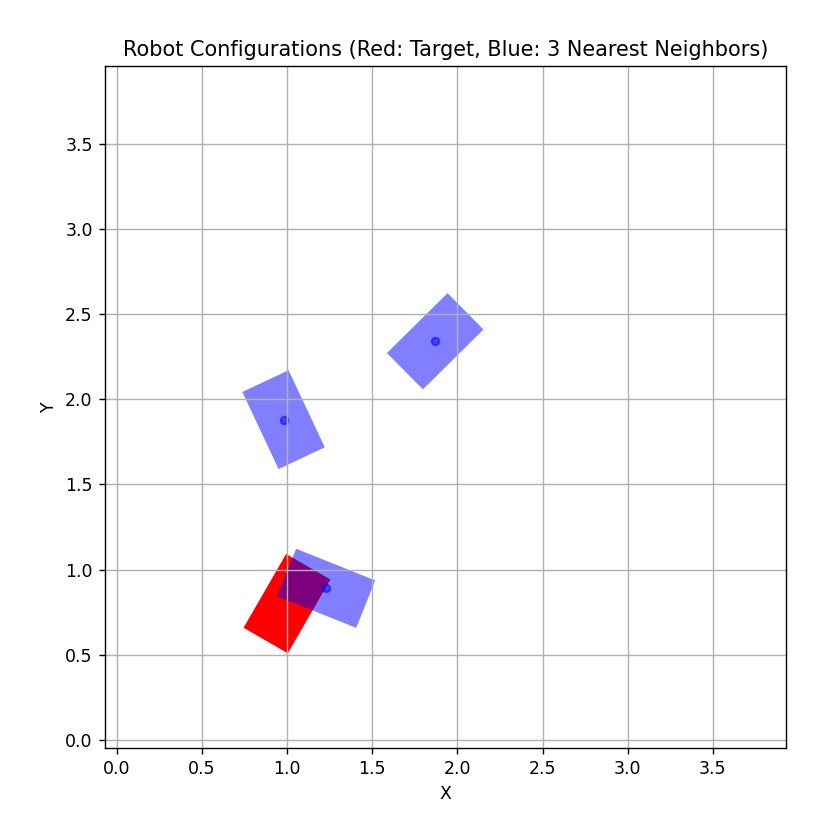
\includegraphics[width=0.5\linewidth]{latex_media/nearestFreeBody2.jpg}
    \caption{Query: (1.0, 0.8, 1.04)
    Nearest configurations: [(1.23, 0.89, 2.76), (0.98, 1.88, 2.01), (1.87, 2.34, 0.78)]}
\end{figure}

\begin{figure} [H]
    \centering
    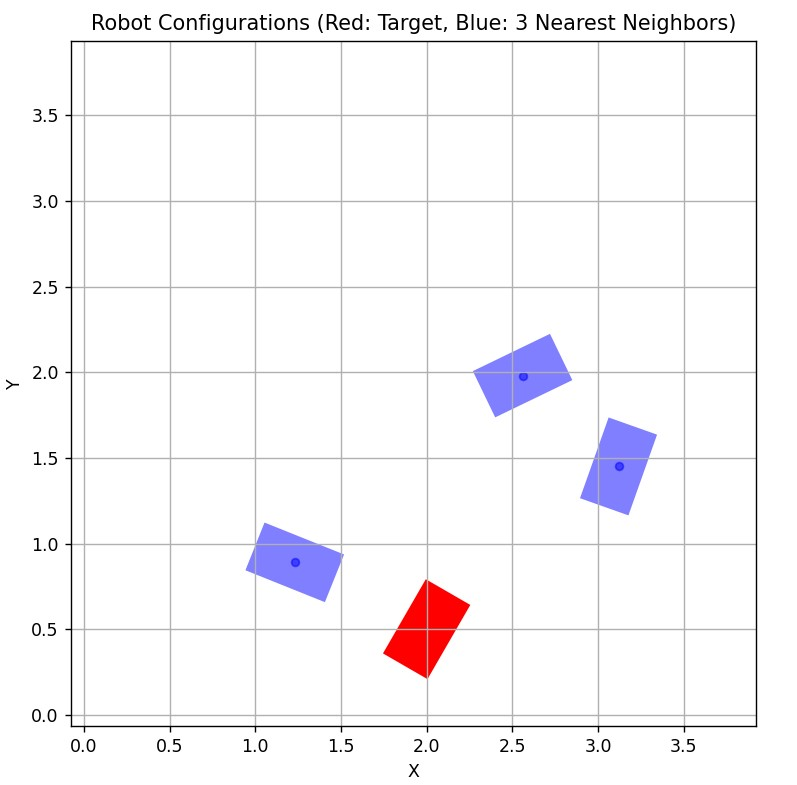
\includegraphics[width=0.5\linewidth]{latex_media/nearestFreeBody3.jpg}
    \caption{Query: (2.0, 0.5, 1.04)
    Nearest configurations: [(3.12, 1.45, 1.23), (1.23, 0.89, 2.76), (2.56, 1.98, 0.45)]}
\end{figure}

\section{Collision Checking}

The idea for collision checking here is using SAT or the separating axis theorem, similar to the one we used to generate the environments to ensure the obstacles wouldn't overlap. First, it gets the corners of the obstacle in the environment and then applies it to a rotation matrix to get the rotated corners. Next, it gets the normal vectors to the edges of the obstacle (got the edges from the corners just calculated) and stores them as potential separating axes. Next, the robot's and the obstacle's corners are projected onto each axis in a loop. There is no collision if the projections do not overlap on at least one axis. This is repeated for each obstacle in the environment for each configuration generated. Below you will see the process run on all 5 environments for free body and arm. For the arm, we centered it at (10,10) so that it could reach all around without going out of bounds. For the visualizing, we found the end effector's angle and placed the rectangle of (0.5,0.3) at that position and orientation to check for collisions. This process is run for ten poses each time. (This code can be run with arguments)

\begin{figure} [H]
    \centering
    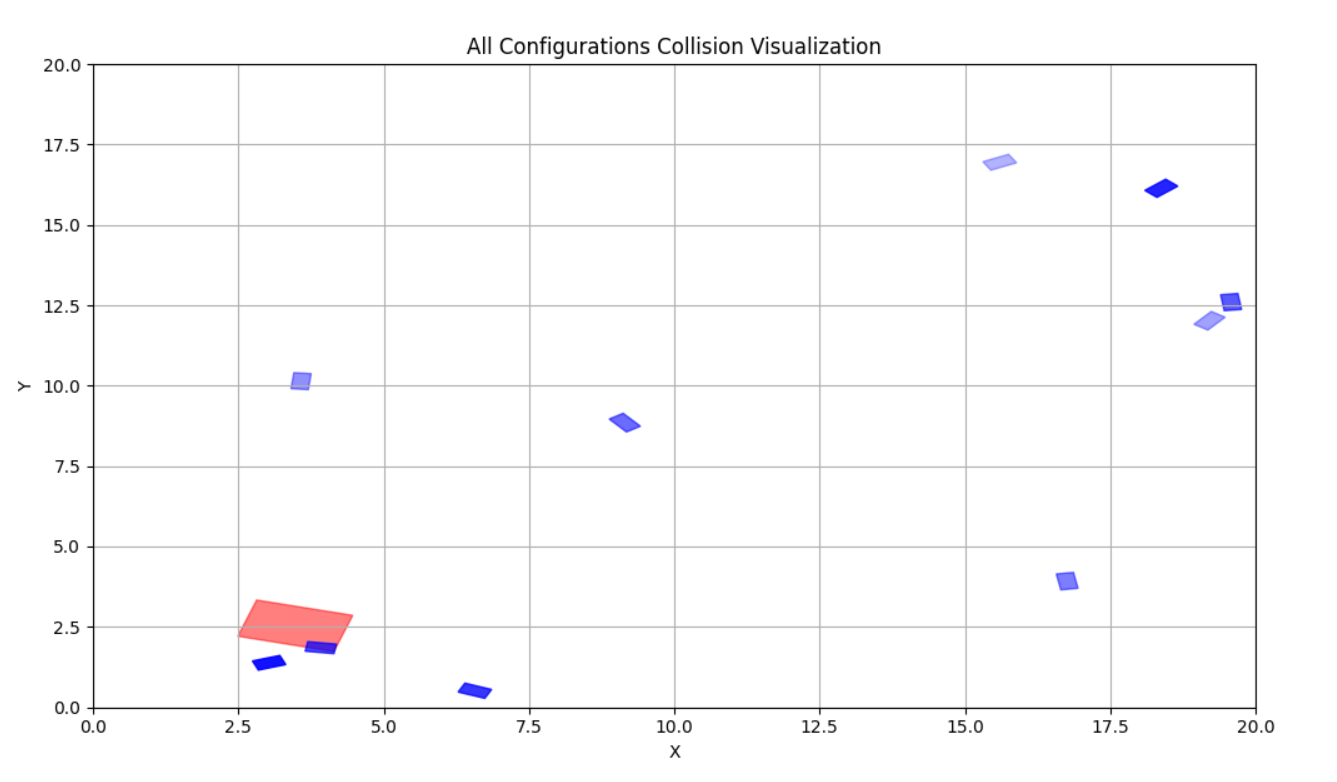
\includegraphics[width=0.7\linewidth]{latex_media/config_collision_freebody_env1.png}
    \caption{Free body configurations with Environment 1}
\end{figure}

\begin{figure} [H]
    \centering
    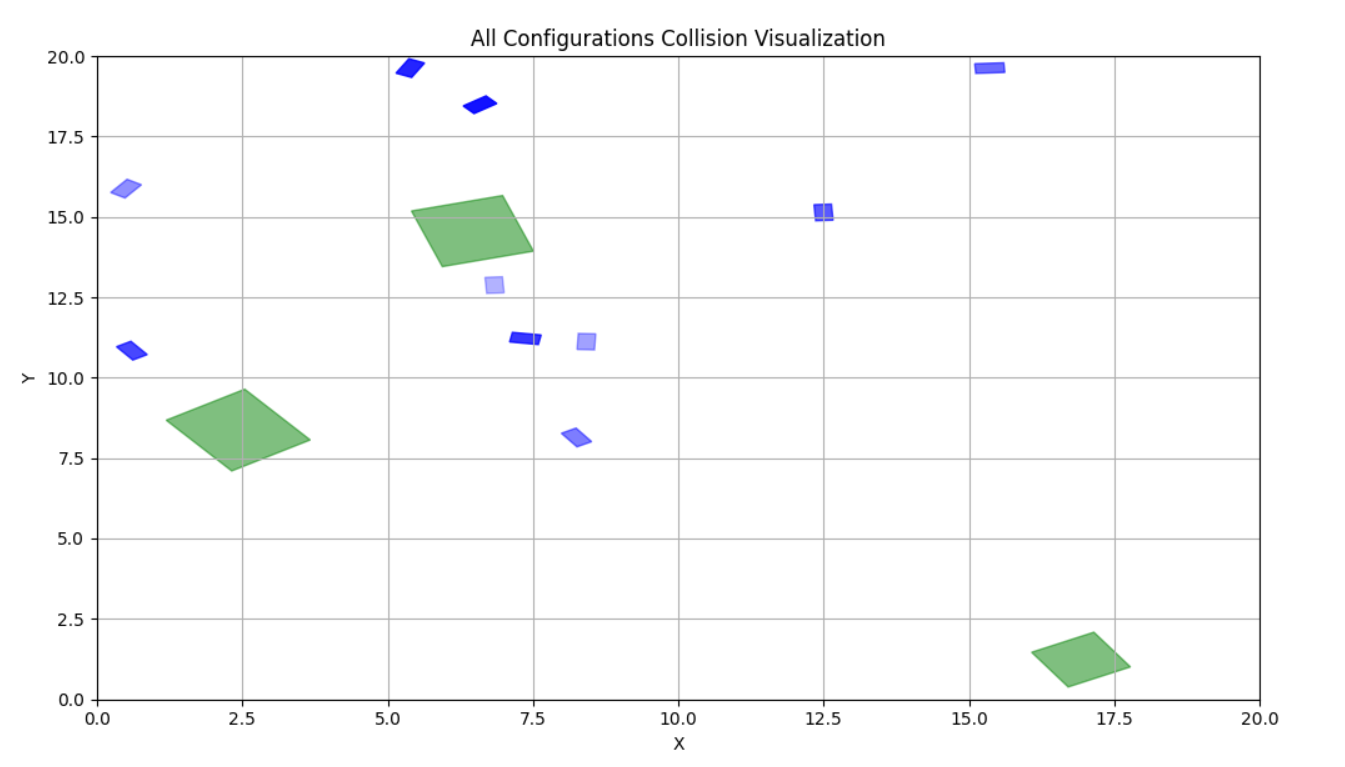
\includegraphics[width=0.7\linewidth]{latex_media/config_collision_freebody_env2.png}
    \caption{Free body configurations with Environment 2}
\end{figure}

\begin{figure} [H]
    \centering
    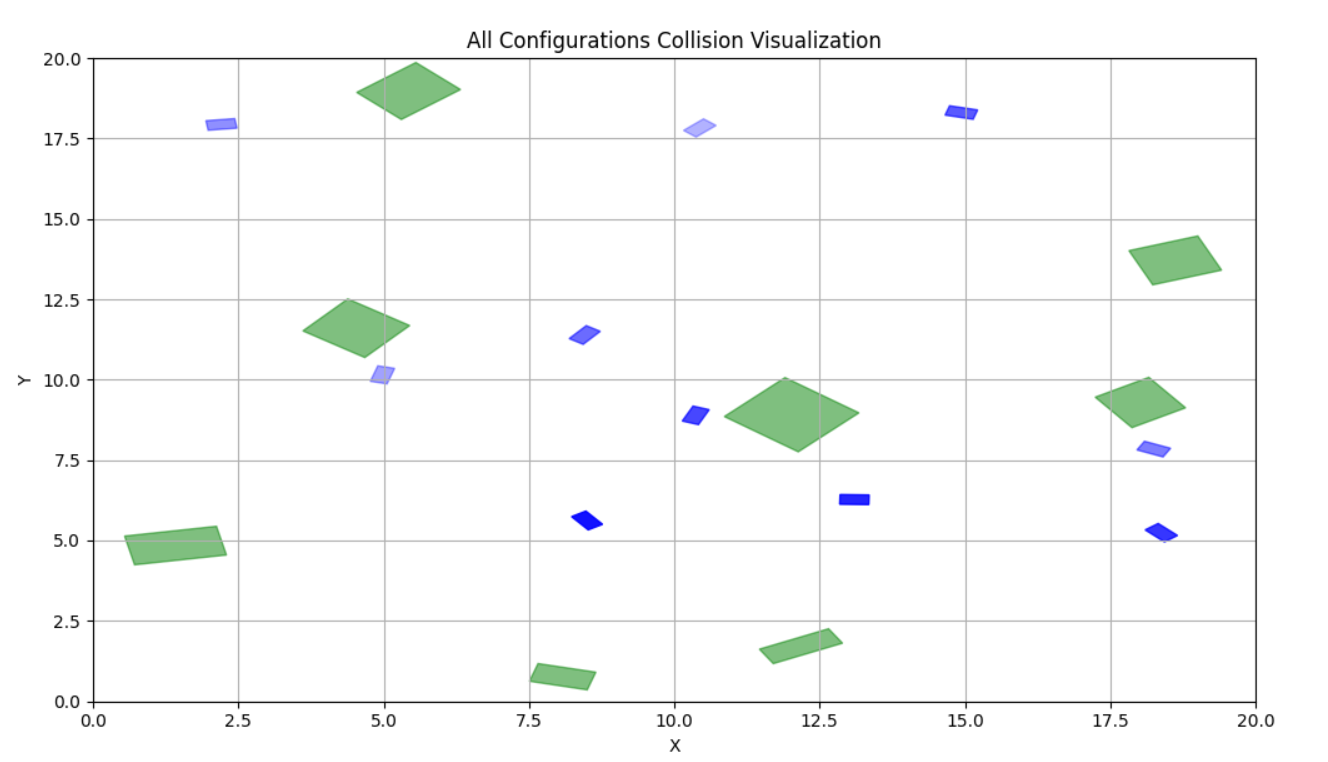
\includegraphics[width=0.7\linewidth]{latex_media/config_collision_freebody_env3.png}
    \caption{Free body configurations with Environment 3}
\end{figure}

\begin{figure} [H]
    \centering
    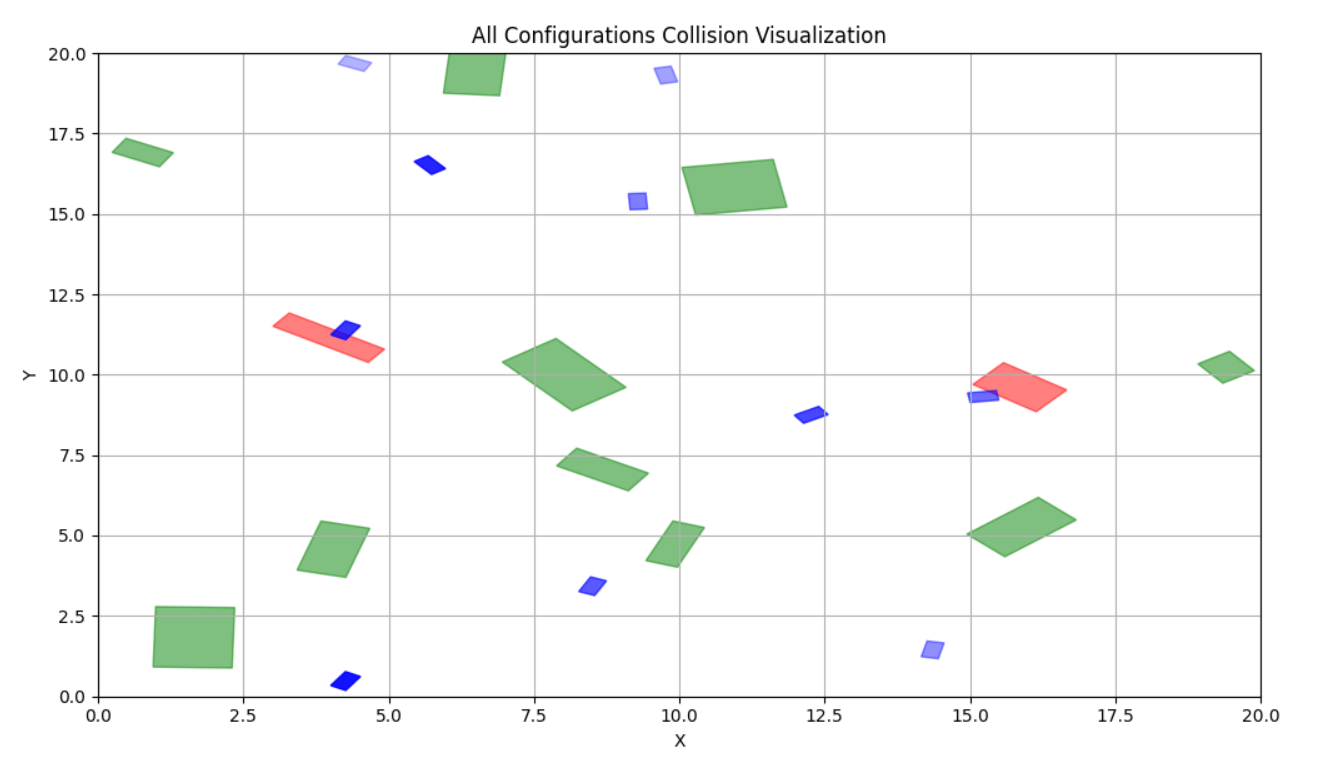
\includegraphics[width=0.7\linewidth]{latex_media/config_collision_freebody_env4.png}
    \caption{Free body configurations with Environment 4}
\end{figure}

\begin{figure} [H]
    \centering
    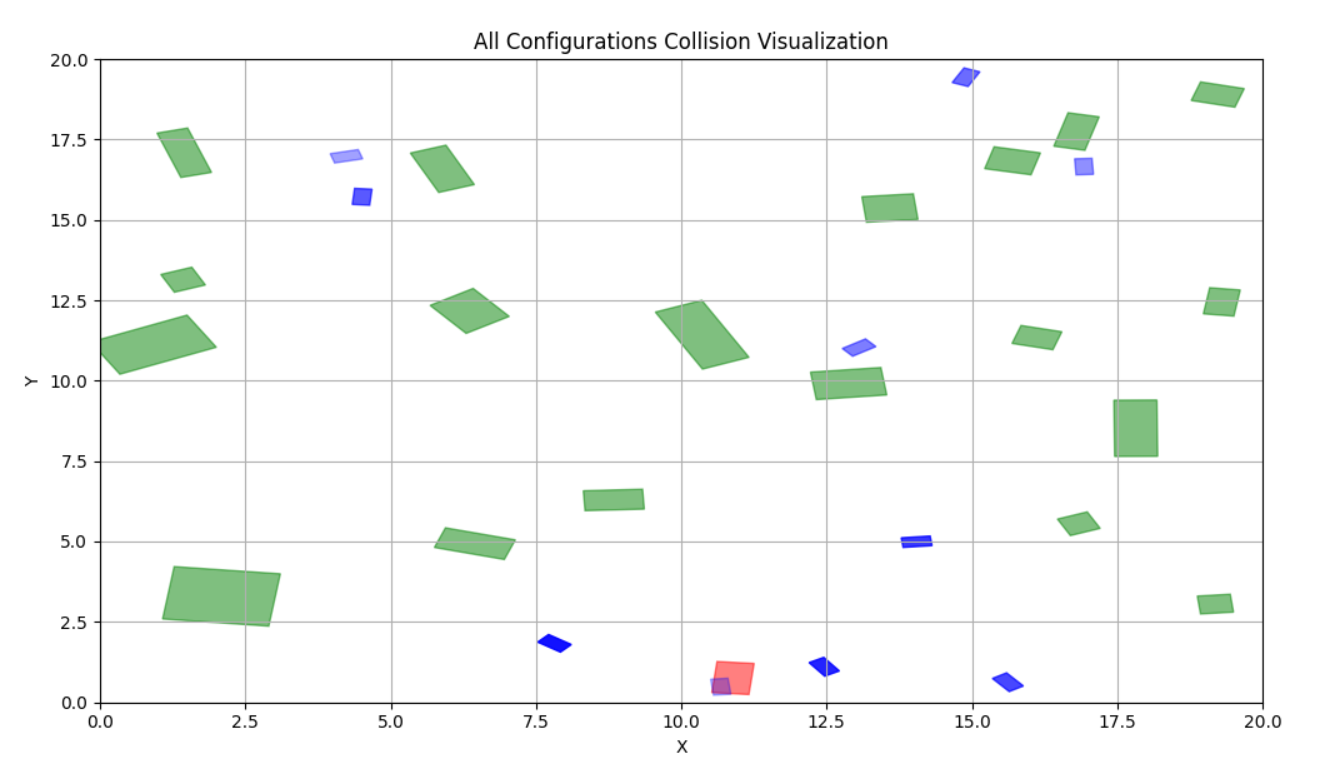
\includegraphics[width=0.7\linewidth]{latex_media/config_collision_freebody_env5.png}
    \caption{Free body configurations with Environment 5}
\end{figure}

\begin{figure} [H]
    \centering
    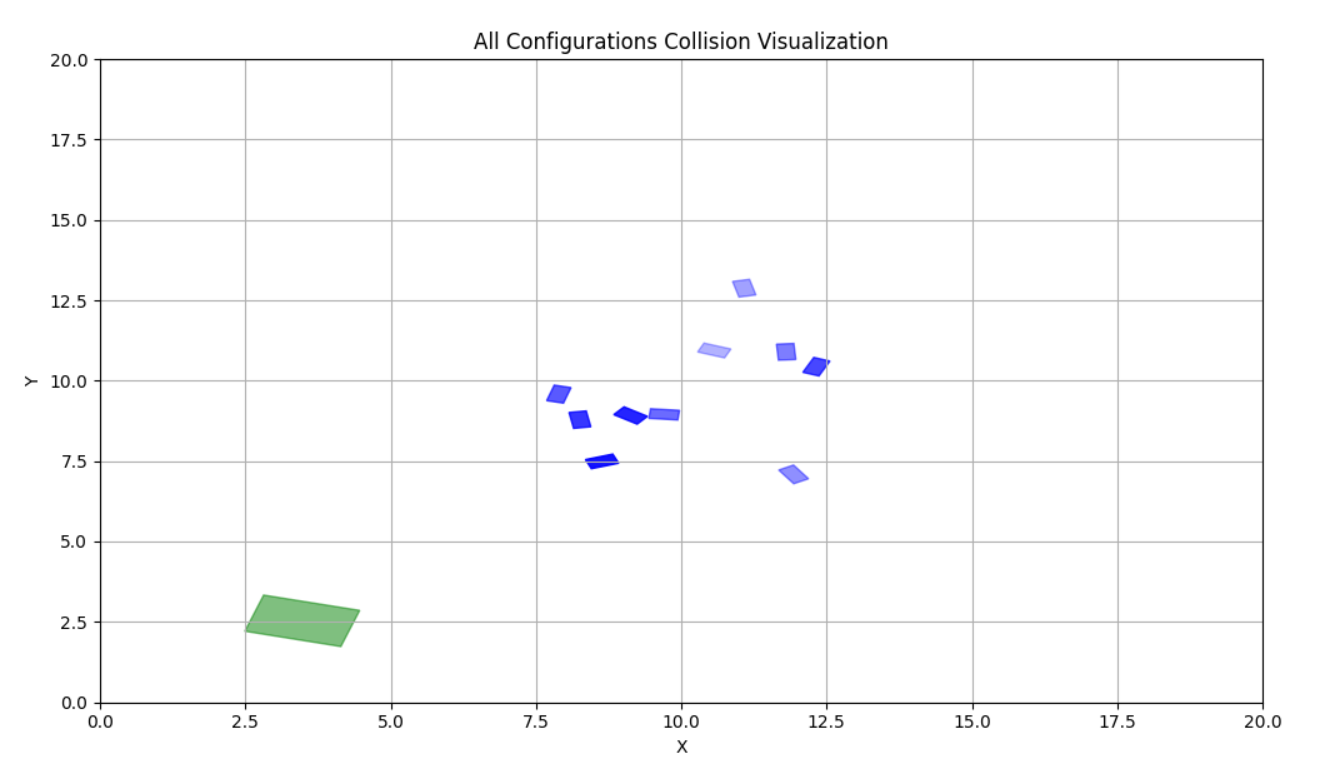
\includegraphics[width=0.7\linewidth]{latex_media/config_collision_arm_env1.png}
    \caption{Arm configurations with Environment 1}
\end{figure}

\begin{figure} [H]
    \centering
    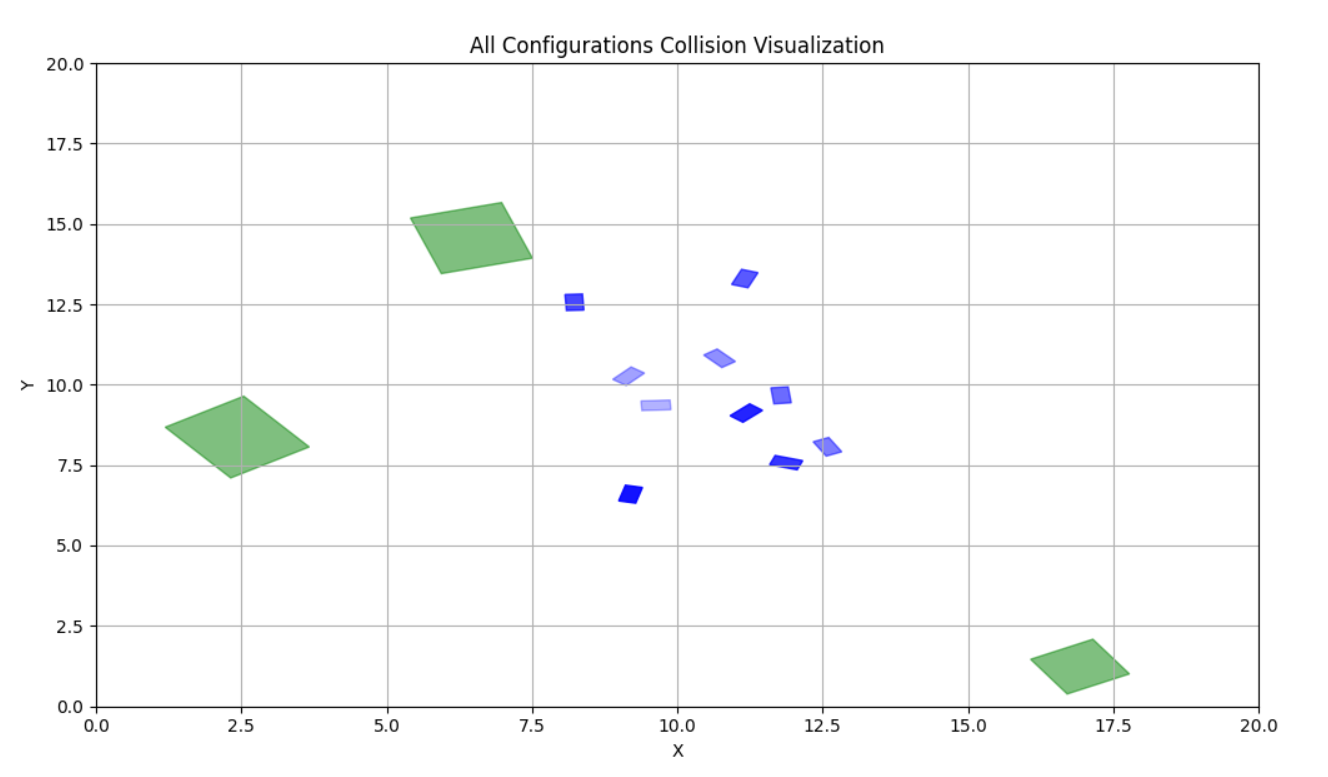
\includegraphics[width=0.7\linewidth]{latex_media/config_collision_arm_env2.png}
    \caption{Arm configurations with Environment 2}
\end{figure}

\begin{figure} [H]
    \centering
    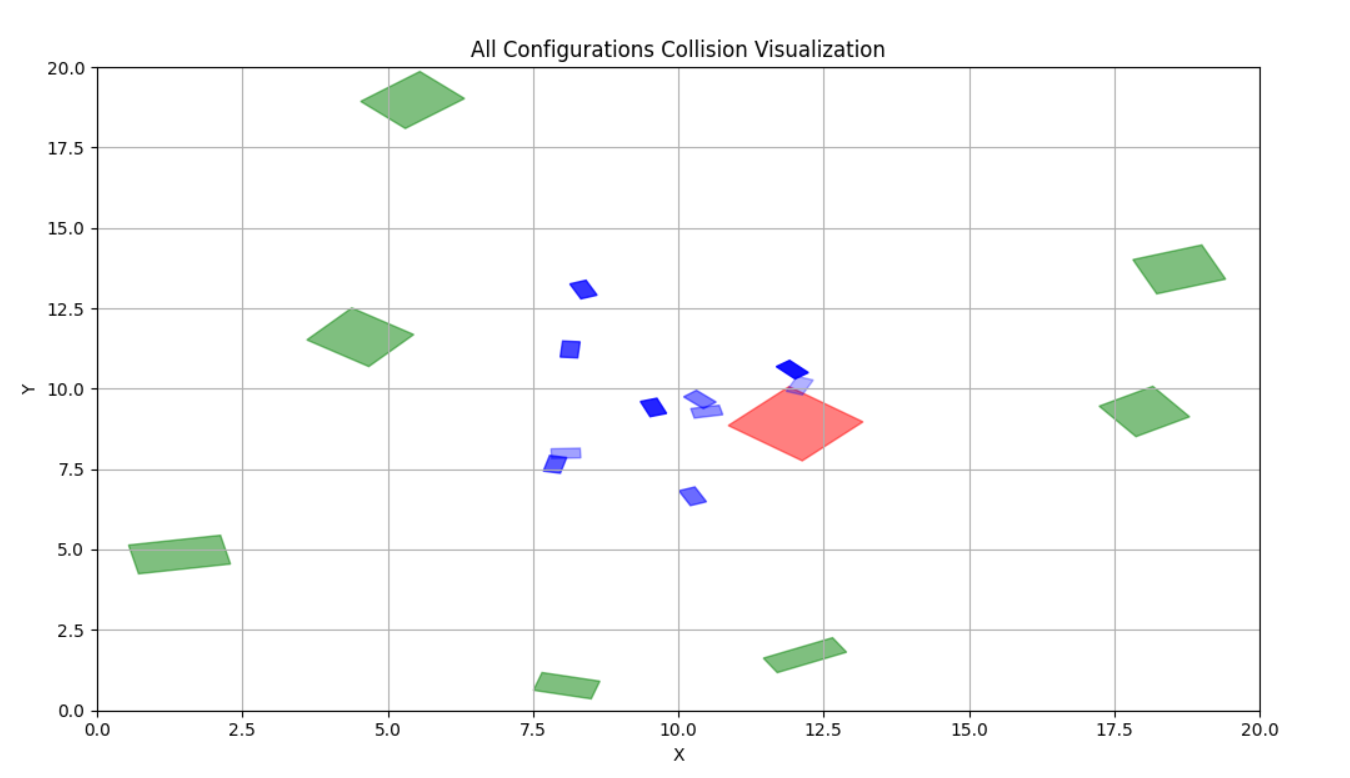
\includegraphics[width=0.7\linewidth]{latex_media/config_collision_arm_env3.png}
    \caption{Arm configurations with Environment 3}
\end{figure}

\begin{figure} [H]
    \centering
    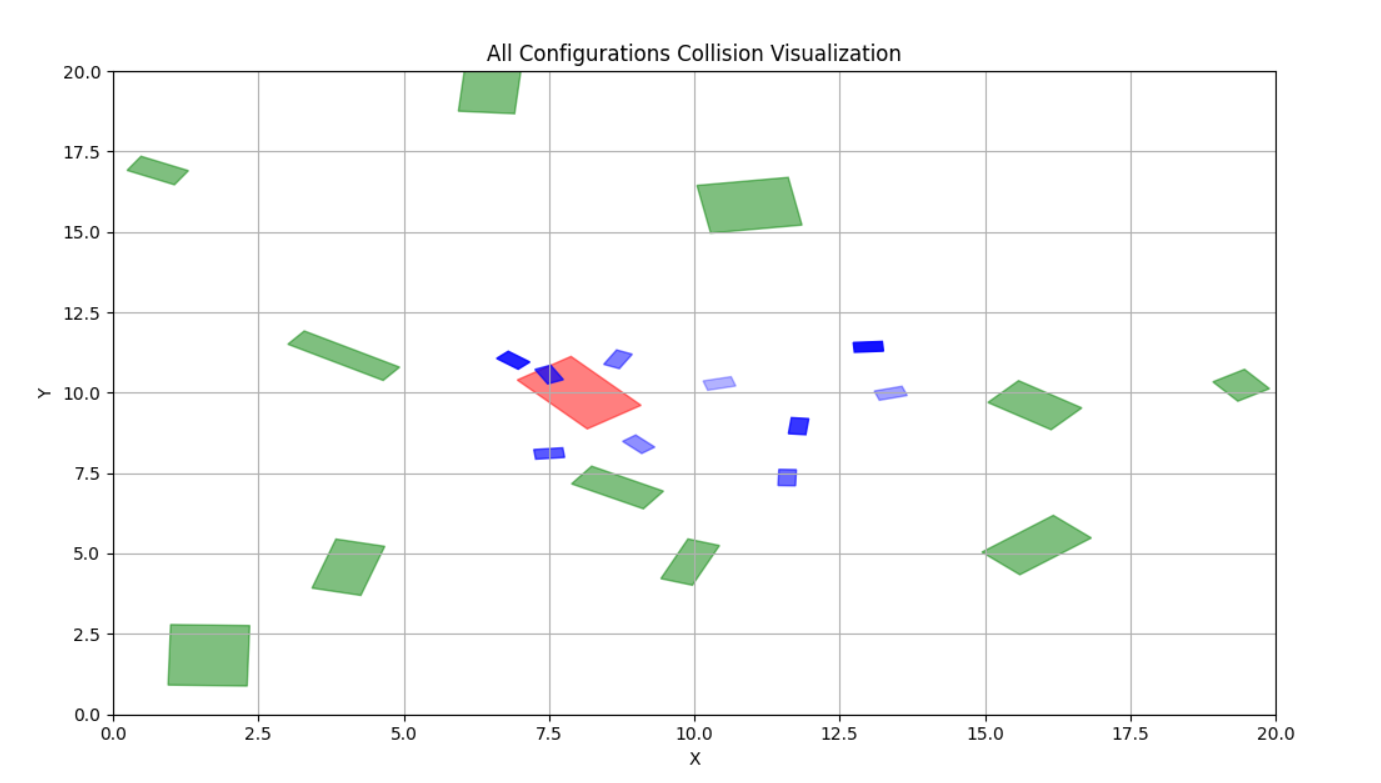
\includegraphics[width=0.7\linewidth]{latex_media/config_collision_arm_env4.png}
    \caption{Arm configurations with Environment 4}
\end{figure}

\begin{figure} [H]
    \centering
    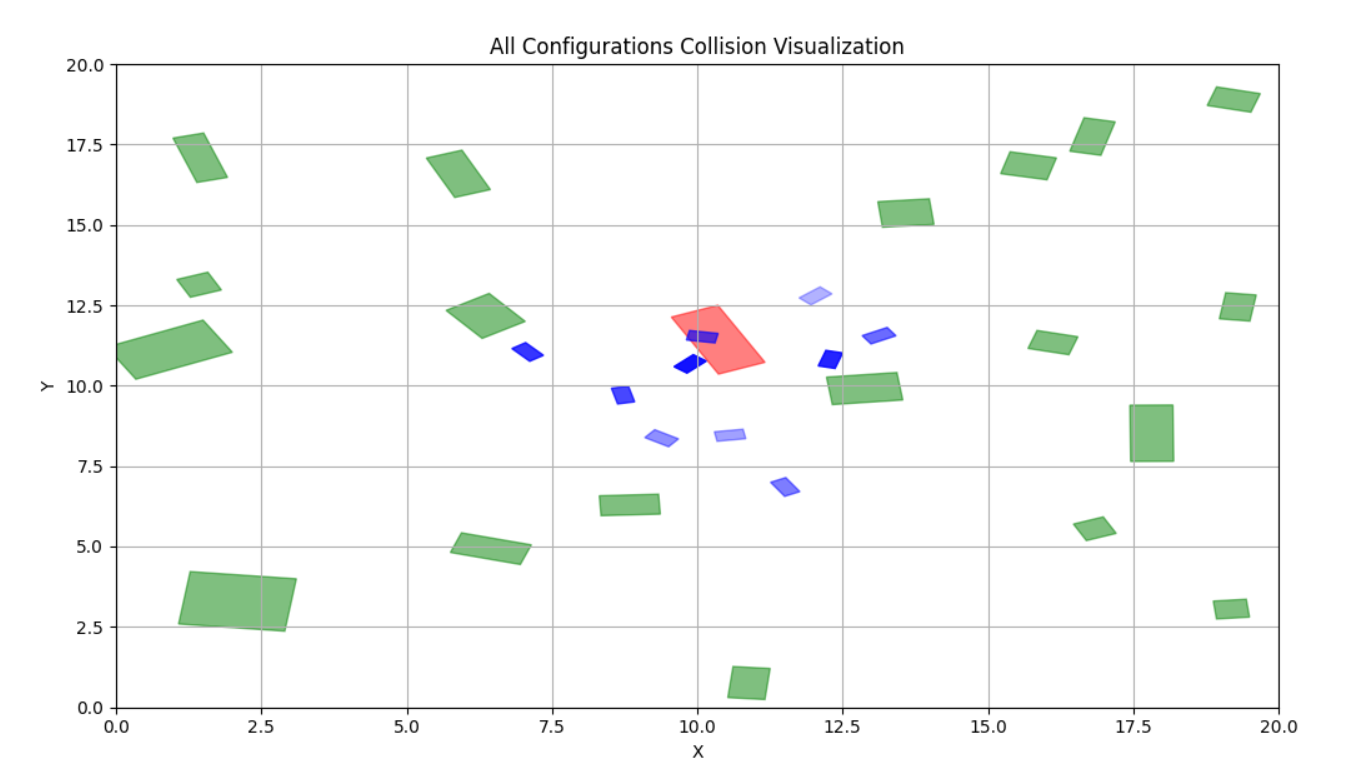
\includegraphics[width=0.7\linewidth]{latex_media/config_collision_arm_env5.png}
    \caption{Arm configurations with Environment 5}
\end{figure}

\section{PRM}

Utilized Node and Object classes for easier object handling. The Node class represented a point in configuration space for the arm or free body. The Obstacle class represented the rectangular obstacles, and it allowed us to get the corners of the obstacle.

To better organize and handle all the functionalities of the Probabilistic Roadmap (PRM) approach, we created the PRMPlanner class. The planner itself has many function definitions, including \texttt{\_\_init\_\_}, \texttt{check\_collision}, \texttt{check\_arm\_collision\_single}, \texttt{build\_roadmap}, and etc. The general workflow follows taking the inputs from the command line argument flags and instantiating a PRMPlanner object with those arguments. Depending on the type of robot, we adapt the dimensions of the robot to fit a free body or an arm (0.5 x 0.3 for the free body and 2 and 1.5 for the link lengths, respectively). From there, the program loads the configurations of all the obstacles from the file into a list of obstacles. Next, the script begins to build the roadmap, which checks if the start and goal configurations are valid, returning an error if they are invalid. After, we will generate some number of configurations as long as the quantity of configurations does not exceed the specified number of samples, which is 5000 in this case. These configurations are sampled randomly and uniformly but have different specifications depending on the type of the robot. As long as these configurations are collision-free, we append these configurations into a list which is then converted to a node through the Node class.

After initializing a KDTree, we attempt to connect these nodes together by iterating through the list of nodes and querying the tree for the nearest neighbors to a particular node. If these neighbors are not already connected to the node and there is no collision between these nodes, then the neighbors are added to the node's list of neighbors. Next, we visualize the roadmap in C-space or the workspace for the arm and the free body, respectively. These visualizations depicted nodes as circles and the connections as lines.

After visualizing the roadmap, the next plan of action is to obtain the path that connects the start and goal configurations together. The \texttt{path} function utilizes the A* search algorithm to find the path from the start configuration to the goal configuration. As long as the path exists, we animate the path from the start configuration of the robot to the end configuration.

\begin{figure} [H]
    \centering
    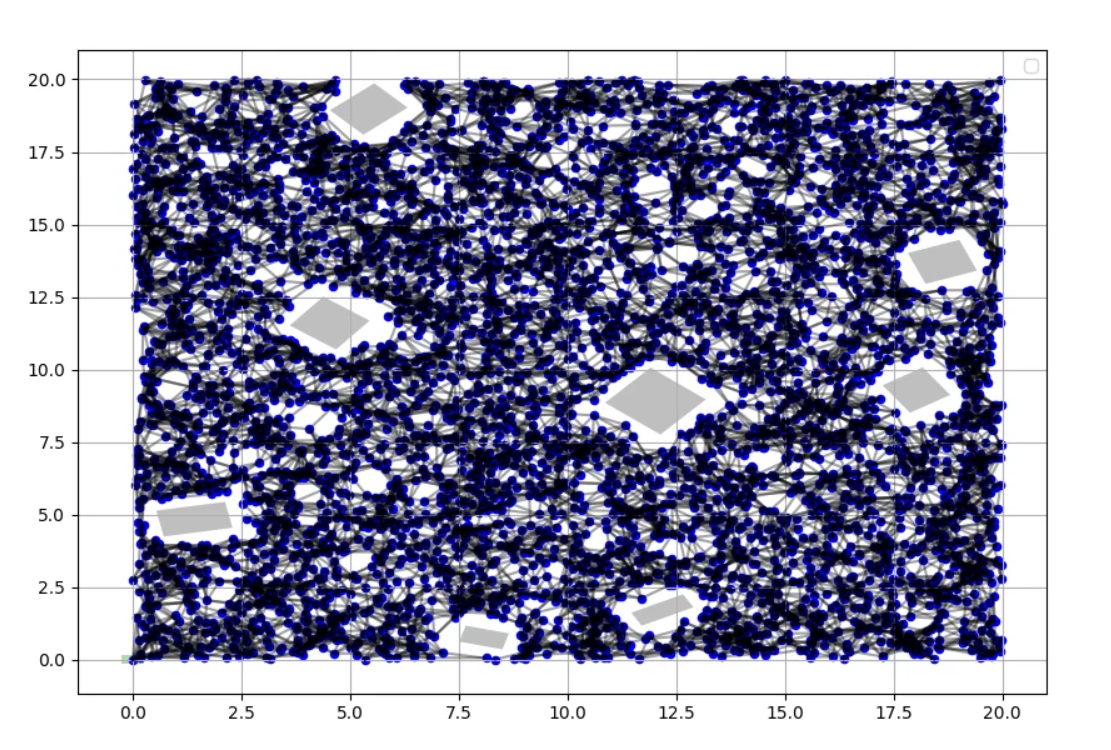
\includegraphics[width=0.7\linewidth]{latex_media/prm_freebody_env3_conf1.png}
    \caption{python3 prm.py --robot freeBody --start 0 0 0 --goal 16 10 0 --map Env3.txt}
\end{figure}

\begin{figure} [H]
    \centering
    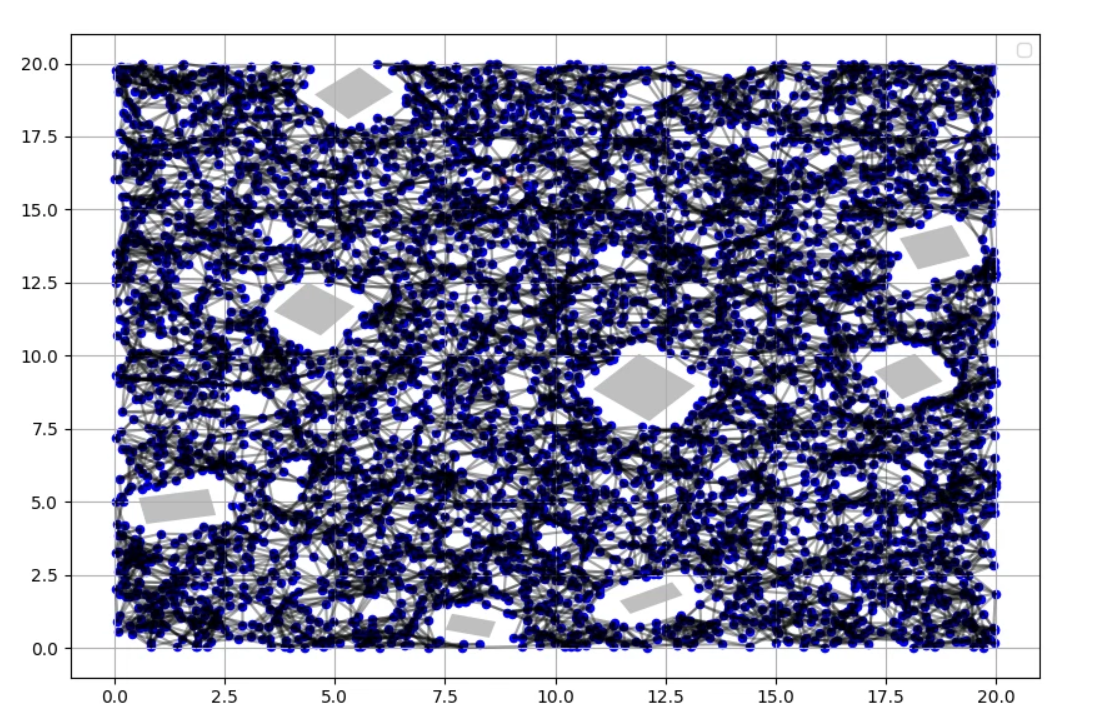
\includegraphics[width=0.7\linewidth]{latex_media/prm_freebody_env3_conf2.png}
    \caption{python3 prm.py --robot freeBody --start 2 10 0 --goal 9 16 0 --map Env3.txt}
\end{figure}

\begin{figure} [H]
    \centering
    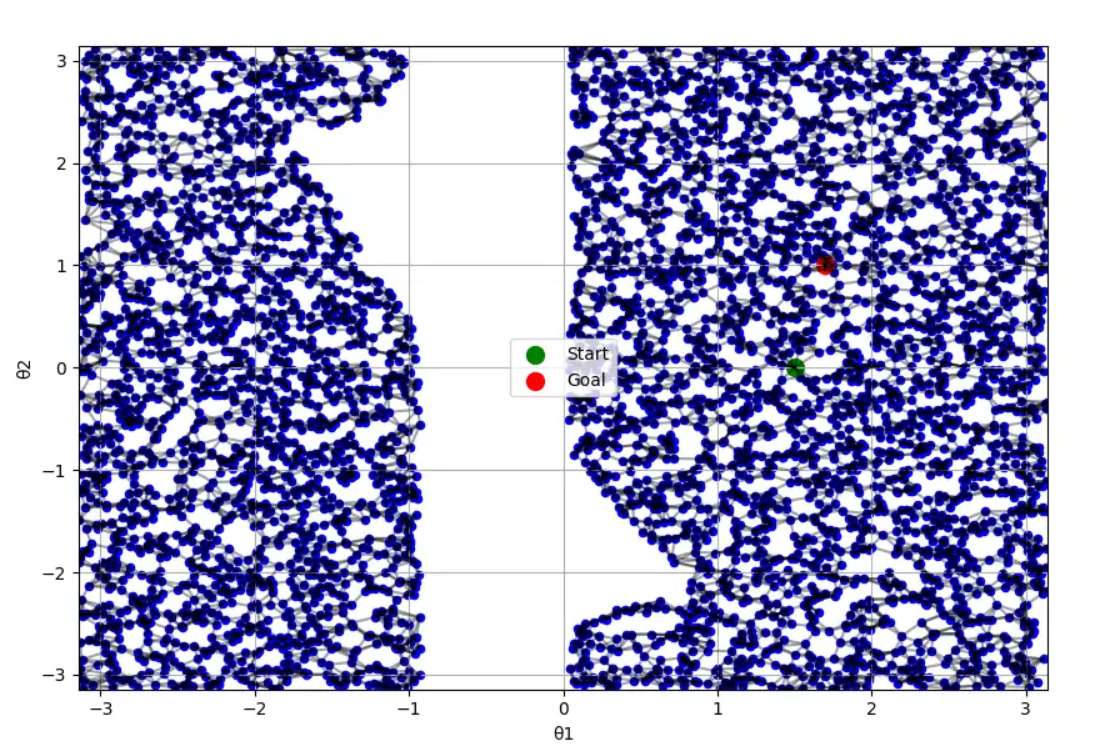
\includegraphics[width=0.7\linewidth]{latex_media/prm_arm_env3_conf1.png}
    \caption{python3 prm.py --robot arm --start 1.5 0 --goal 1.7 1 --map Env3.txt}
\end{figure}

\begin{figure} [H]
    \centering
    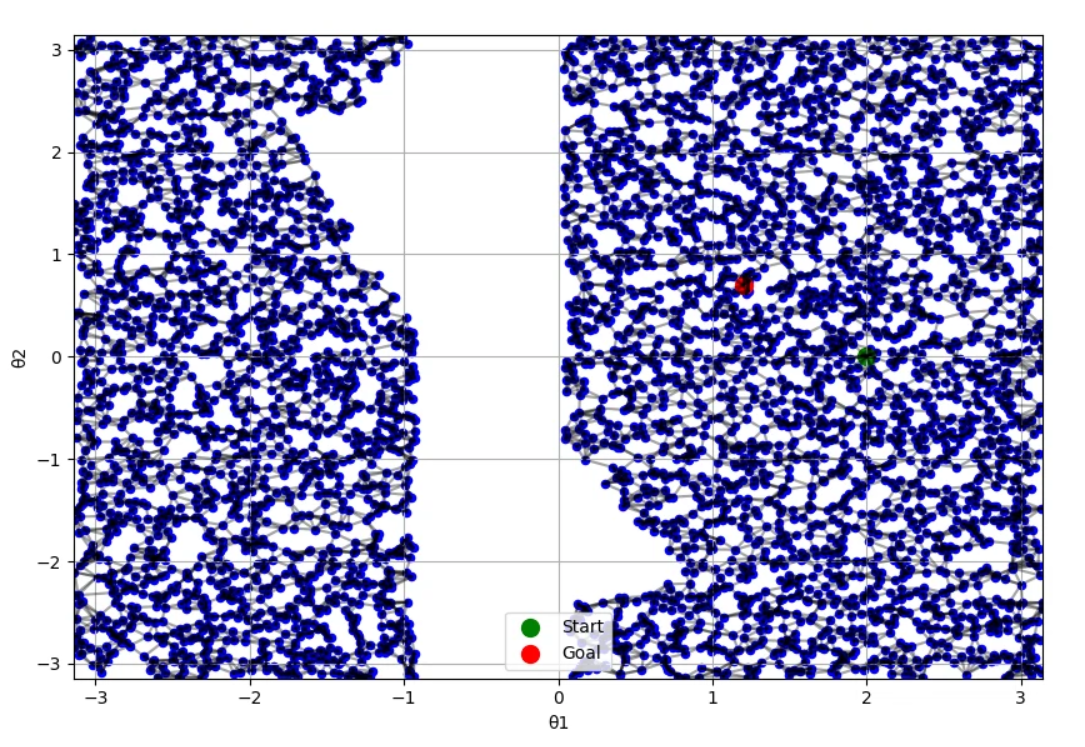
\includegraphics[width=0.7\linewidth]{latex_media/prm_arm_env3_conf2.png}
    \caption{python3 prm.py --robot arm --start 2 0 --goal 1.2 0.7 --map Env3.txt}
\end{figure}

\begin{figure} [H]
    \centering
    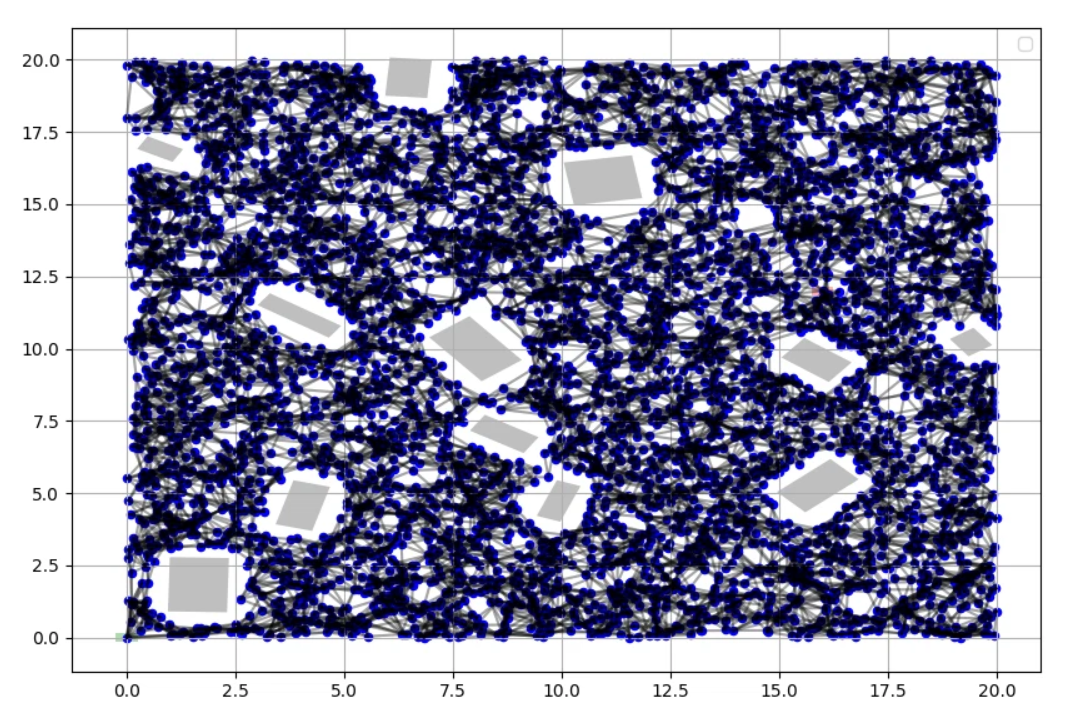
\includegraphics[width=0.7\linewidth]{latex_media/prm_freebody_env4_conf1.png}
    \caption{python3 prm.py --robot freeBody --start 0 0 0 --goal 16 12 0 --map Env4.txt}
\end{figure}

\begin{figure} [H]
    \centering
    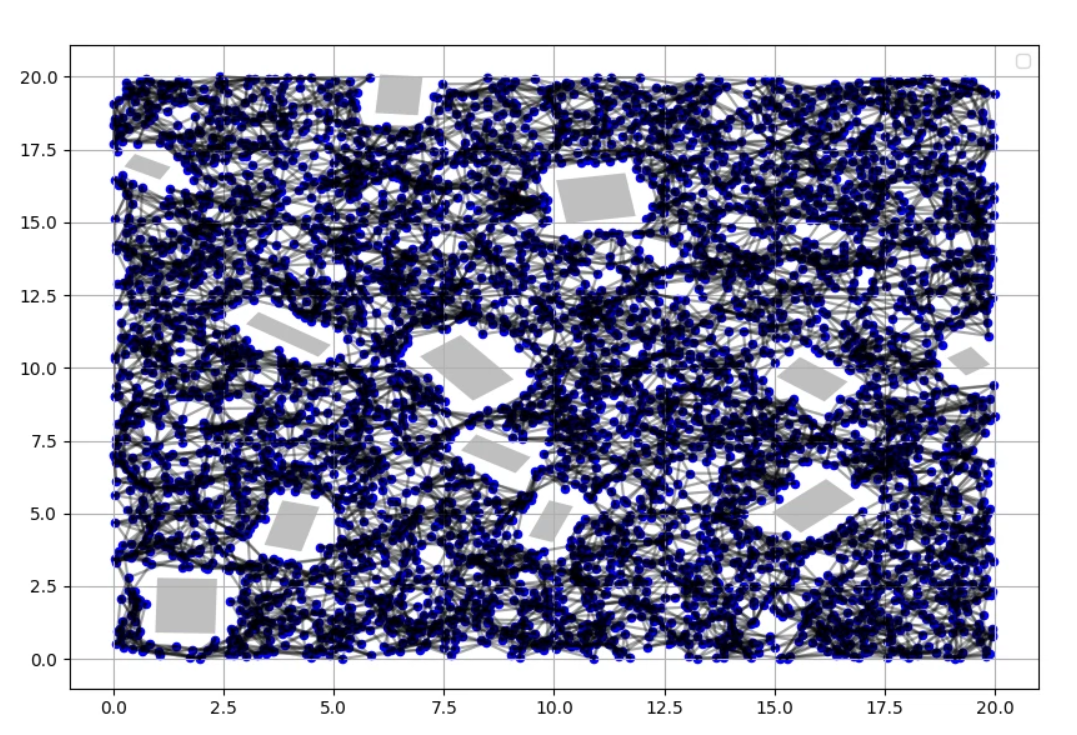
\includegraphics[width=0.7\linewidth]{latex_media/prm_freebody_env4_conf2.png}
    \caption{python3 prm.py --robot freeBody --start 2 10 0 --goal 9 16 0 --map Env4.txt}
\end{figure}

\begin{figure} [H]
    \centering
    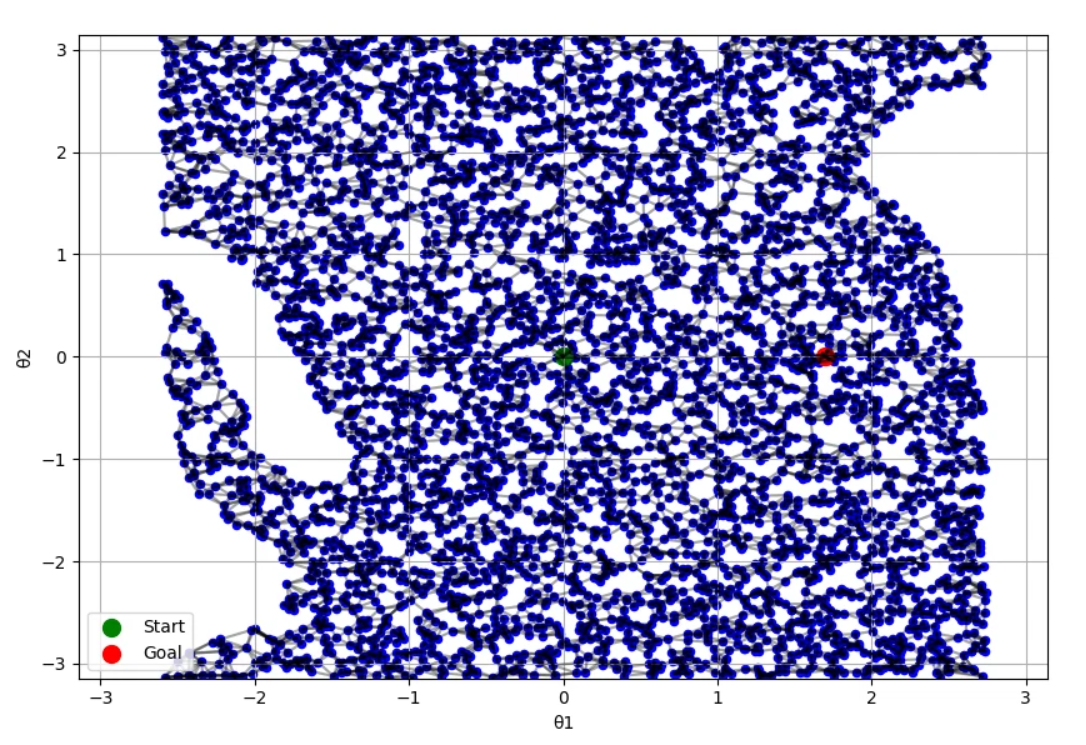
\includegraphics[width=0.7\linewidth]{latex_media/prm_arm_env4_conf1.png}
    \caption{python3 prm.py --robot arm --start 0 0 --goal 1.7 0 --map Env4.txt
}
\end{figure}

\begin{figure} [H]
    \centering
    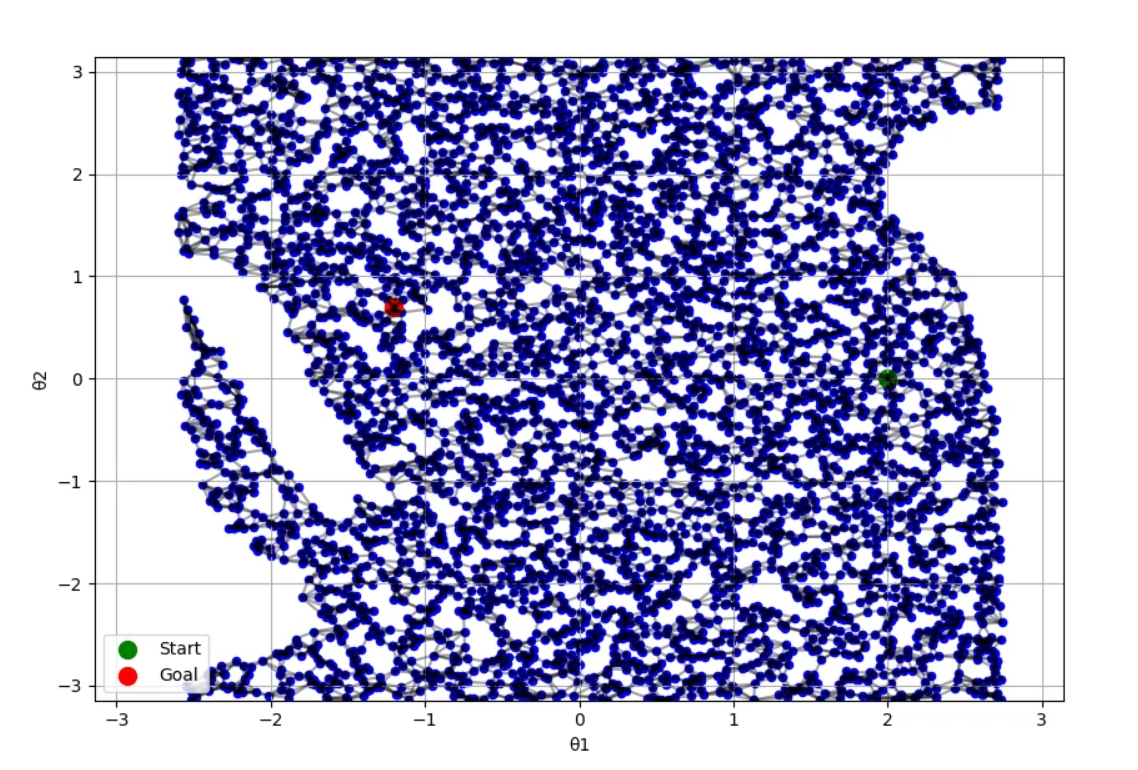
\includegraphics[width=0.7\linewidth]{latex_media/prm_arm_env4_conf2.png}
    \caption{python3 prm.py --robot arm --start 2 0 --goal -1.2 0.7 --map Env4.txt}
\end{figure}

\subsection{Implement RRT}

For the RRT approach, we used the same classes as PRM to construct the Node and Obstacle objects, to hold required information and methods. 
For the actual RRT Planner, we made sure to define the specific dimensions of the robot based on it being a free body or arm (0.5 x 0.3 for the free body and 2 and 1.5 for the link lengths, respectively). Next, after setting up and making sure the start configuration and end configuration are in bounds, it runs the build tree function. It starts the tree at the single node at the start configuration. Here, it samples a random configuration in the allowed c-space for the robot for n number of iterations, or until it has already plotted 1000 nodes for the tree. The random configuration is validated after checking for collisions from obstacles and bounds. Then, the tree will try to extend to this node using the nearest neighbor to it. The nearest neighbor is found by calculating Euclidean distance for the free body or using angular distance for an arm based on our previous code explained earlier. We decided to have our code also encourage branching for nodes that have fewer children so that the tree can cover more ground. After that is decided it steers to the new node, based on a step size we define, and it calculates how much to move, and then we recheck the new configuration in between the current and random configuration to make sure it stays in bounds. If the new node configuration we found is too close to the current position we don't add to eliminate space needed to store this node. Specifically for the C-space, checking for the edge, we split for the freebody and arm. For the free body collision checking function, we get the corners of the robot and obstacle and check if the edge of the robot intersects with the obstacle edge using the segment intersection test over an interpolation between the configurations (used the counterclockwise test to determine if three points make CCW turn if the slope of AC is greater than AB). For the arm, do something similar. In this case, we interpolate between the configurations, loop through these, and get points for the arm segments. Next, we check if any of the points in the segment are in the obstacles by casting a ray to the right of the point. If the ray intersects edges an even number of times, it's on the outside; if it's odd, it's inside the obstacle. This makes sure the edges connecting the nodes are collision-free based on the robot used. After adding the node, we check if we reached the goal by seeing if the position is in the goal radius, and then we also check if the distance between the node and goal is collision-free since it could just be in the circle across an obstacle. We update our progress tracking so that we can print out what iteration, nodes, distance, and closest distance to the goal we are at currently. (Note the labels are not there for the workspace, but they are supposed to be x and y for the free body and workspace plots same as the environment figures from earlier) (The animations are in the folder and they have the same names as the pictures, ex. Env3RobotPathA1 means arm robot solution animation for environment 3, and tree growth is for tree generation)

\begin{figure} [H]
    \centering
    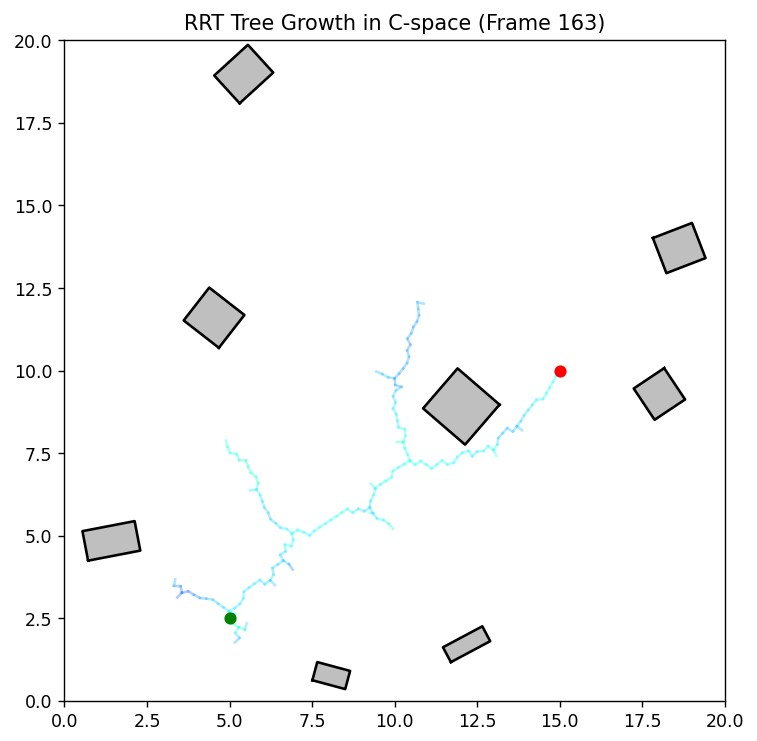
\includegraphics[width=0.5\linewidth]{latex_media/Env3TreeGrowthFB1.jpg}
    \caption{Iteration 180, nodes: 163, --robot freeBody --start 5 2.5 0 --goal 15 10 0 --goal\_rad 0.1 --map Env3.txt}
\end{figure}

\begin{figure} [H]
    \centering
    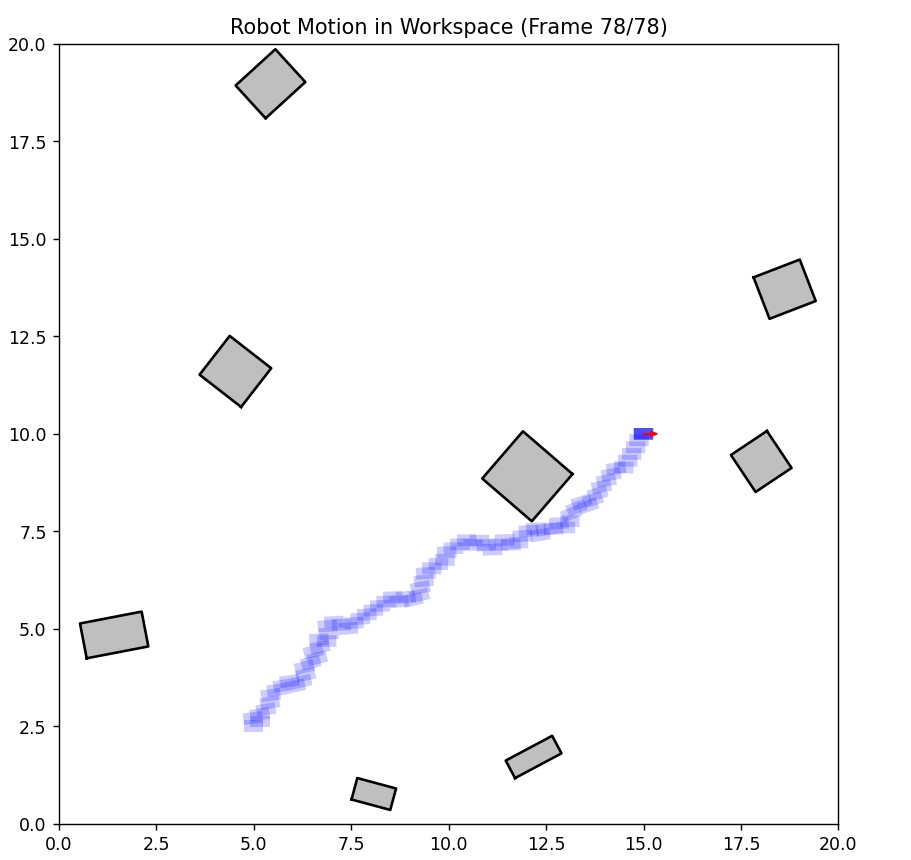
\includegraphics[width=0.5\linewidth]{latex_media/Env3RobotPathFB1.jpg}
    \caption{Environment 3: Freebody Path 1}
\end{figure}

\begin{figure} [H]
    \centering
    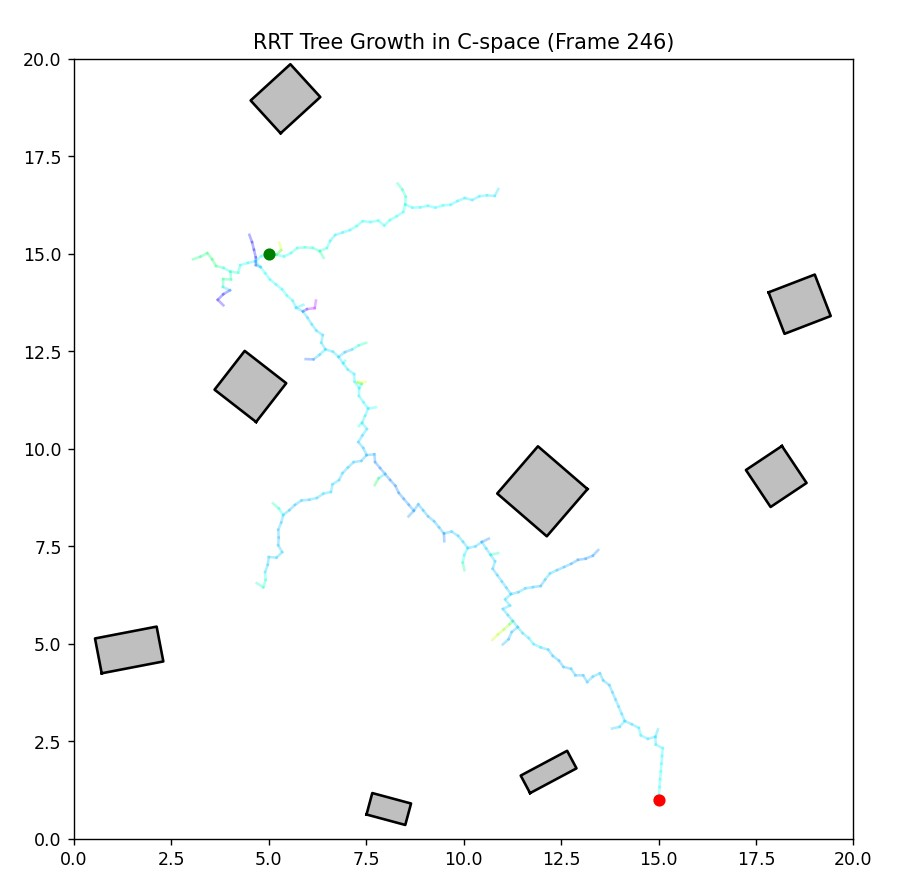
\includegraphics[width=0.5\linewidth]{latex_media/Env3TreeGrowthFB2.jpg}
    \caption{Iteration 245, nodes: 246, --robot freeBody --start 5 15 0 --goal 15 1 0 --goal\_rad 0.1 --map Env3.txt}
\end{figure}

\begin{figure} [H]
    \centering
    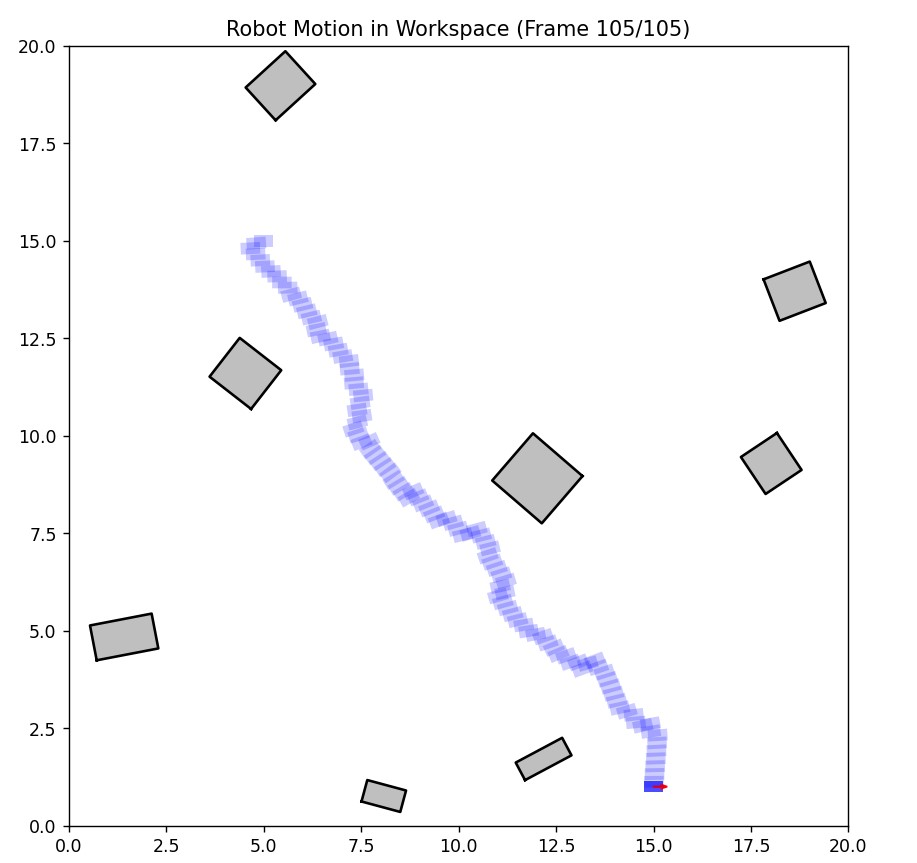
\includegraphics[width=0.5\linewidth]{latex_media/Env3RobotPathFB2.jpg}
    \caption{Environment 3: Freebody Path 2}
\end{figure}

\begin{figure} [H]
    \centering
    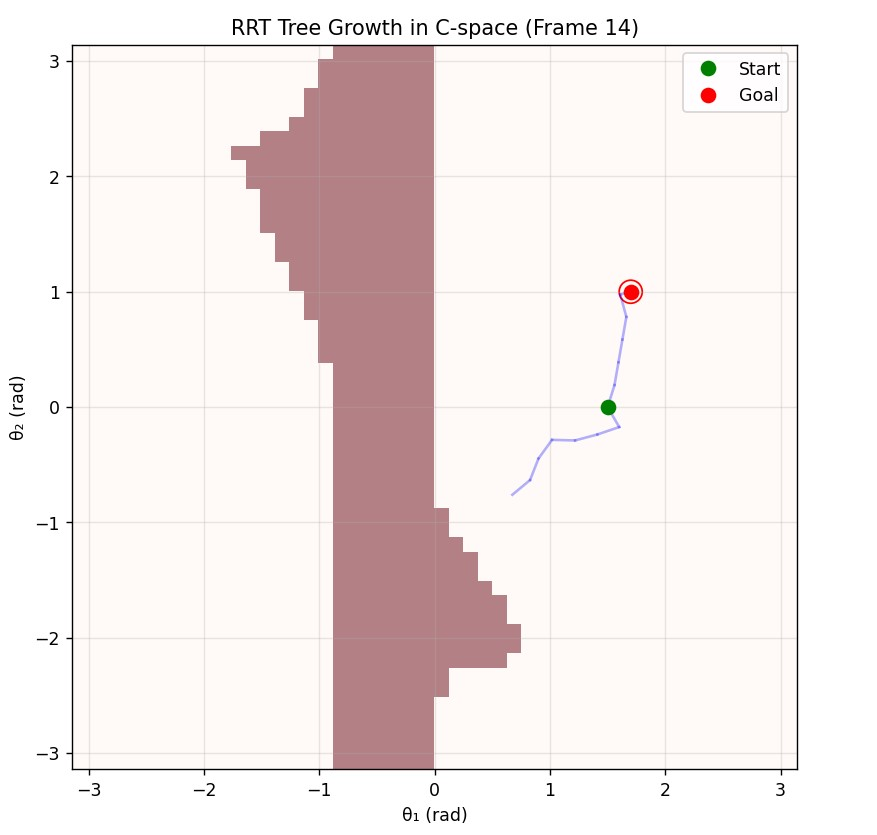
\includegraphics[width=0.5\linewidth]{latex_media/Env3TreeGrowthA1.jpg}
    \caption{Iteration 14, nodes: 14, --robot arm --start 1.5 0 --goal 1.7 1 --goal\_rad 0.1 --map Env3.txt}
\end{figure}

\begin{figure} [H]
    \centering
    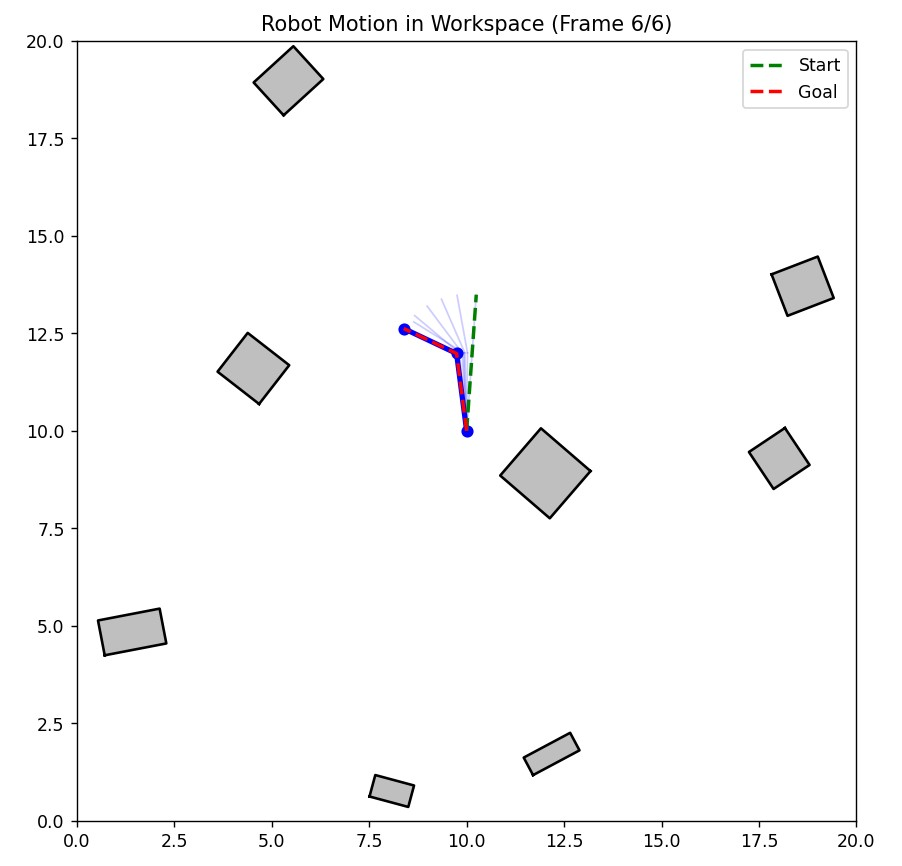
\includegraphics[width=0.5\linewidth]{latex_media/Env3RobotPathA1.jpg}
    \caption{Environment 3: Arm Path 1}
\end{figure}

\begin{figure} [H]
    \centering
    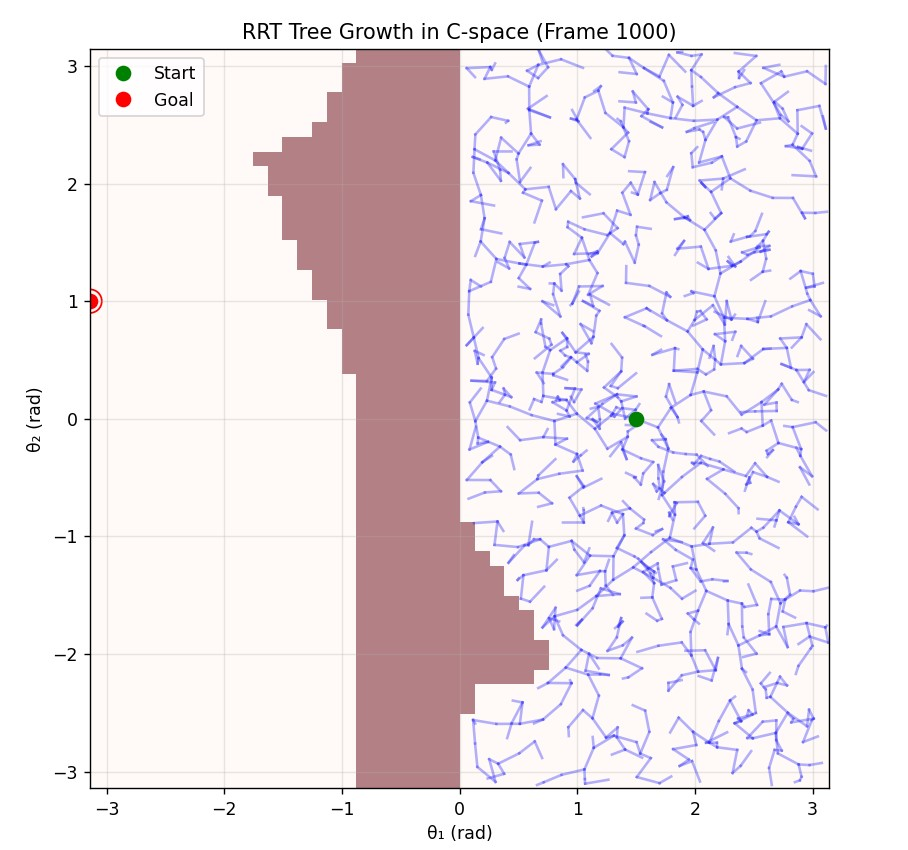
\includegraphics[width=0.5\linewidth]{latex_media/Env3TreeGrowthA2.jpg}
    \caption{Iteration:2641, Nodes:1000, --robot arm --start 1.5 0 --goal -7 1 --goal\_rad 0.1 --map Env3.txt }
\end{figure}

\begin{figure} [H]
    \centering
    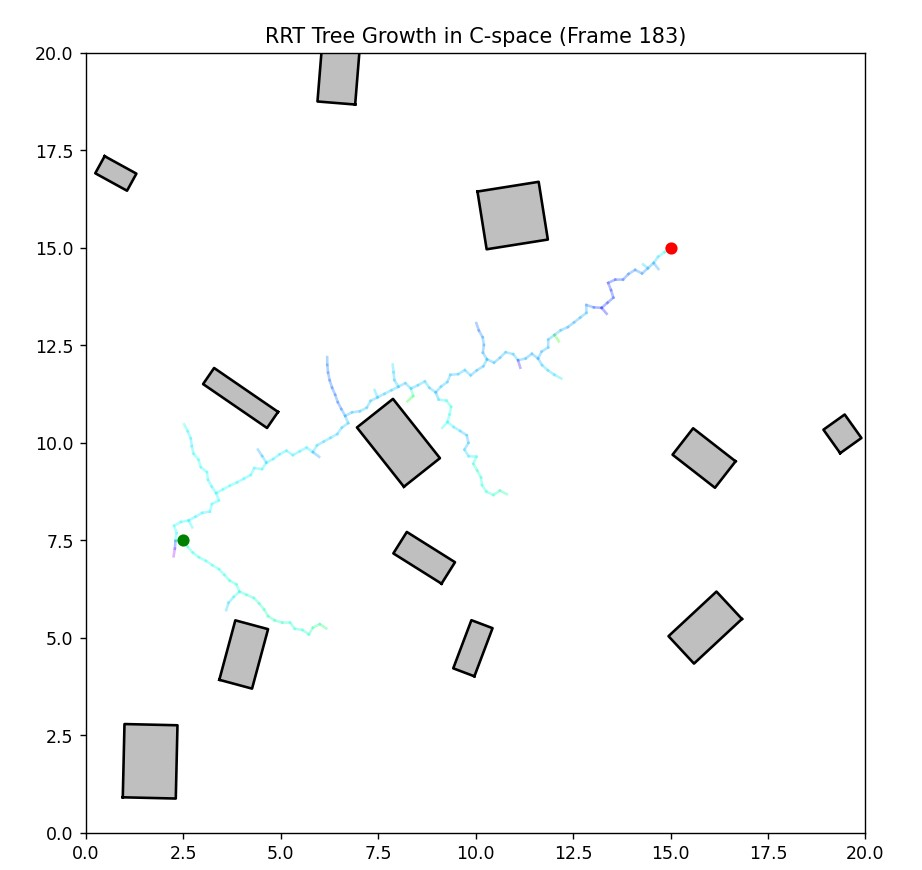
\includegraphics[width=0.5\linewidth]{latex_media/Env4TreeGrowthFB1.jpg}
    \caption{Iteration: 210, Nodes: 183, --robot freeBody --start 2.5 7.5  0 --goal 15 15 0 --goal\_rad 0.1 --map Env4.txt}
\end{figure}

\begin{figure} [H]
    \centering
    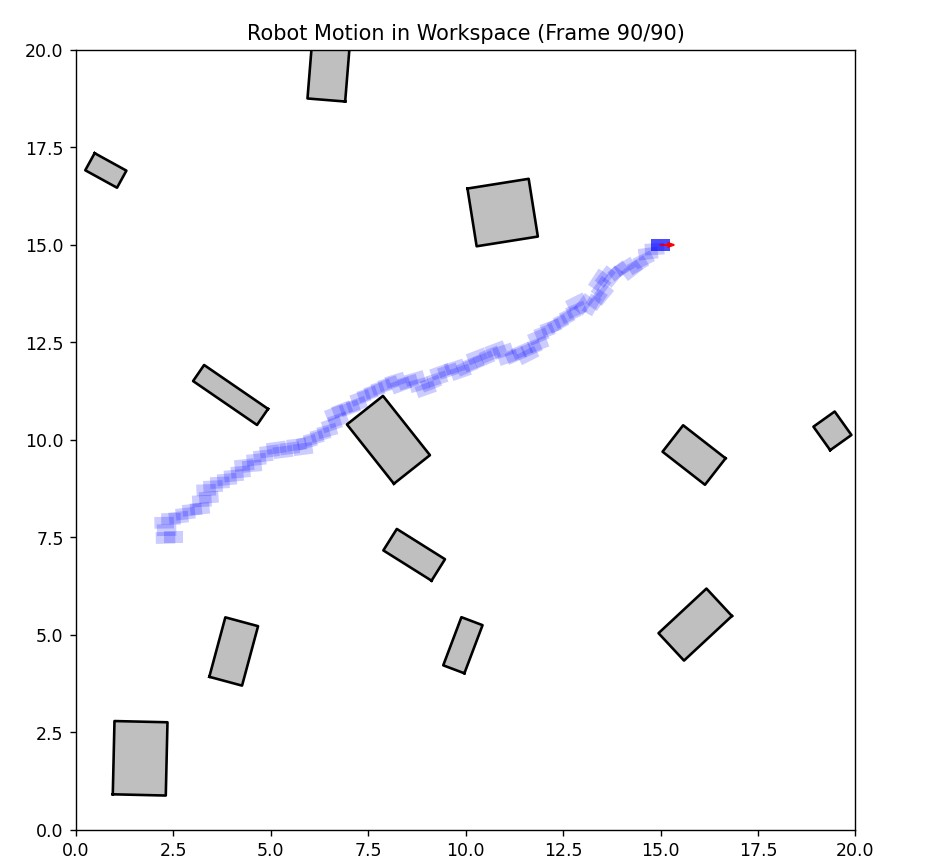
\includegraphics[width=0.5\linewidth]{latex_media/Env4RobotPathFB1.jpg}
    \caption{Environment 4: FreeBody Path 1}
\end{figure}

\begin{figure} [H]
    \centering
    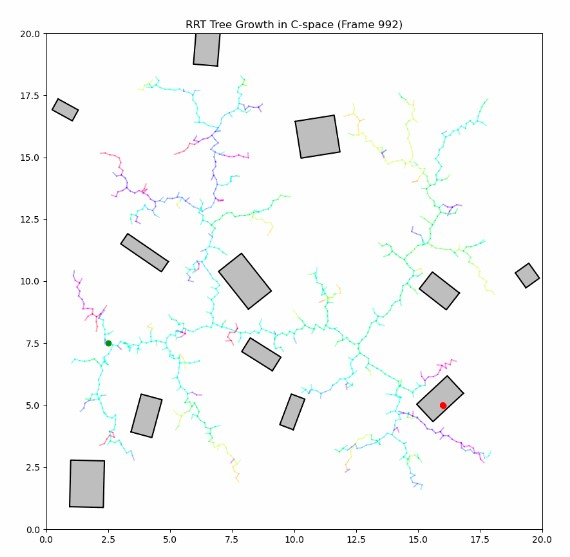
\includegraphics[width=0.5\linewidth]{latex_media/Env4TreeGrowthFB2.jpg}
    \caption{Iteration: 1200, Nodes:1000, --robot freeBody --start 2.5 7.5  0 --goal 16 5 0 --goal\_rad 0.1 --map Env4.txt}
\end{figure}

\begin{figure} [H]
    \centering
    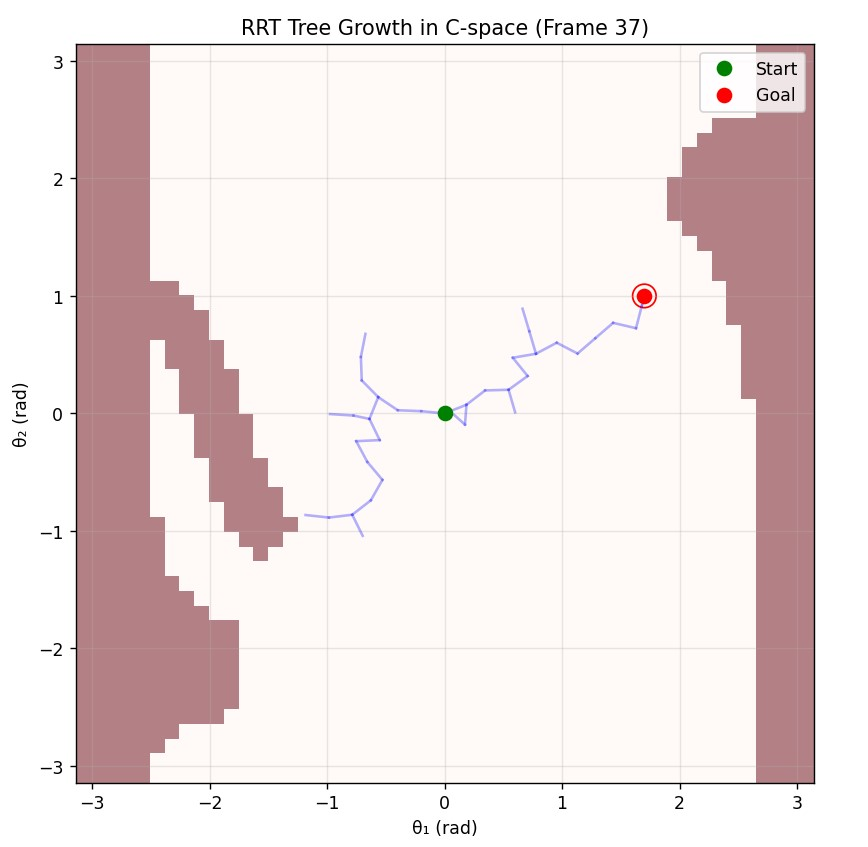
\includegraphics[width=0.5\linewidth]{latex_media/Env4TreeGrowthA1.jpg}
    \caption{Iteration: 35, Nodes: 37, --robot arm --start 0 0 --goal 1.7 1 --goal\_rad 0.1 --map Env4.txt}
\end{figure}

\begin{figure} [H]
    \centering
    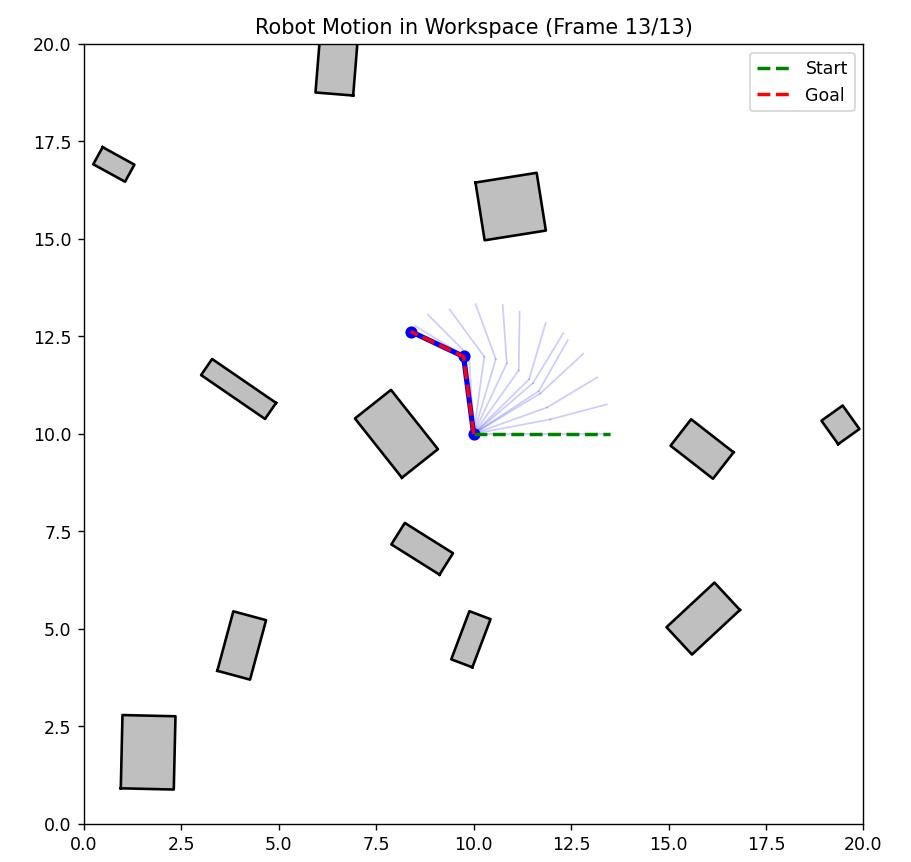
\includegraphics[width=0.5\linewidth]{latex_media/Env4RobotPathA1.jpg}
    \caption{Environment 4: Arm Path 1}
\end{figure}

\begin{figure} [H]
    \centering
    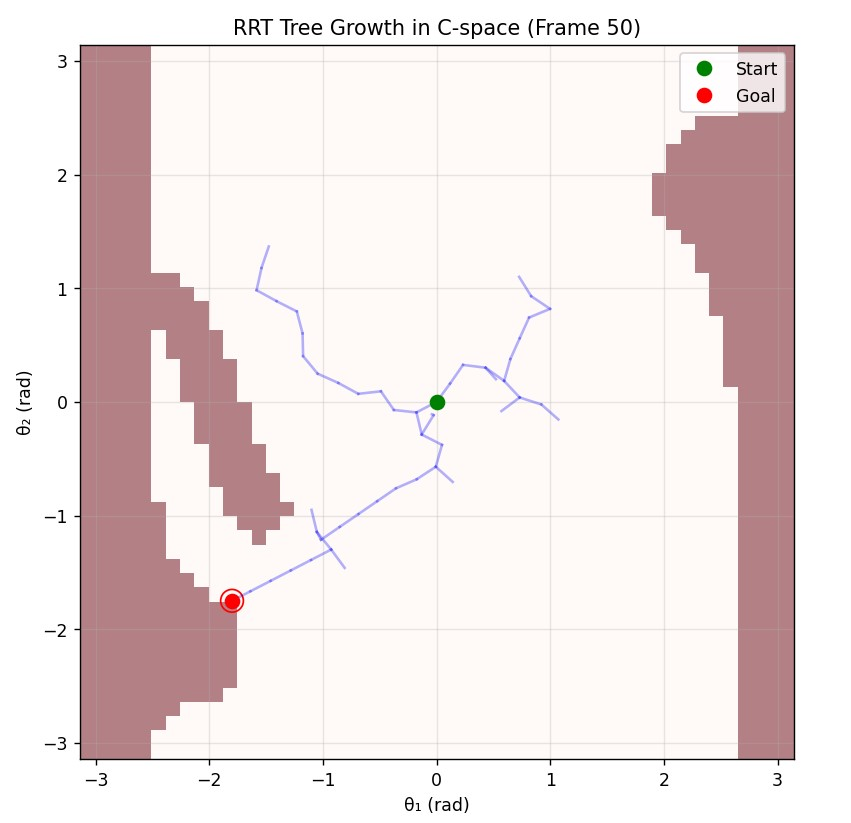
\includegraphics[width=0.5\linewidth]{latex_media/Env4TreeGrowthA2.jpg}
    \caption{Iteration: 48, Nodes: 50, --robot arm --start 0 0 --goal -1.8 -1.8 --goal\_rad 0.1 --map Env4.txt }
\end{figure}

\begin{figure} [H]
    \centering
    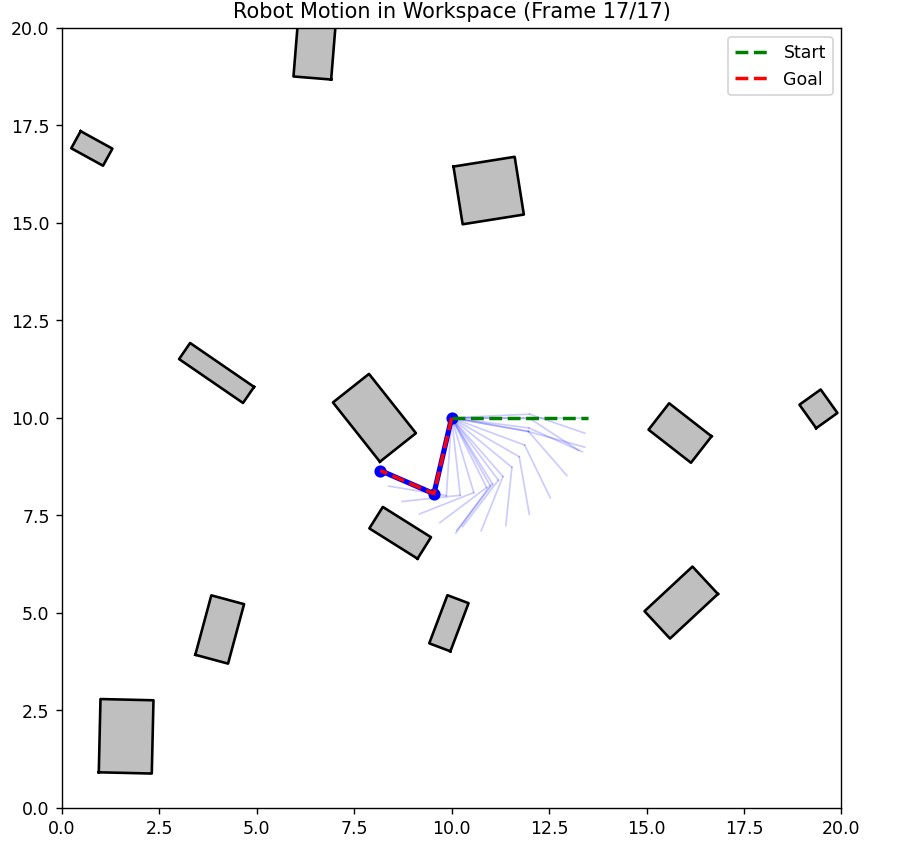
\includegraphics[width=0.5\linewidth]{latex_media/Env4RobotPathA2.jpg}
    \caption{Environment 4: Arm Path 2}
\end{figure}

\section{PRM*/RRT*}
We decided to implement RRT*. We used the same Node class before, but this time, we added a cost for them from the start. The obstacle class remained the same. For the actual RRT* planner in the initialization method, we added a gamma as the tuning parameter that affects the radius that is used when rewiring the nodes to be a more efficient tree. A larger gamma would mean more rewiring at a slower performance, but the path would be more optimal. This gamma is used in addition to the growing samples when calculating the radius. The difference in the extend part of the algorithm is after getting the node to steer for, it checks all the neighbors within a radius and finds the best parent instead of just the closest. It checks with the potential cost we were storing for each node from the start. If no valid, collision-free best parent is found, it reverts back to the old nearest neighbor and uses that. For the rewiring, we check the neighbors and see if the potential new cost of using the new node gives us a better path. If it is, we make sure the segment connection between the new nodes is collision-free and then remove the neighbor from the old parent's children and rewire it through the new node being the parent. We then have to update all the descendant costs of the neighbor with this new node's cost. Another difference here is that we spend time optimizing the path even if we already have found the goal; however, this does cause the algorithm to be slower compared to RRT which is seen in the comparison section. The dynamic radius shrinks as more samples are generated in the nearest neighbor search and the rewiring helps RRT* be asymptotically optimal and not get stuck in local suboptimal paths. 
(Note the labels are the same as the environments above, they are supposed to be x and y for the free body and workspace plots) Had fewer plots here because it takes a long time to animate the gifs. (Same naming convention as before where "Env3AORobotPathFB2" would mean the 2nd free body solution for asymptotic optimal algorithm ran on environment 3)

\begin{figure} [H]
    \centering
    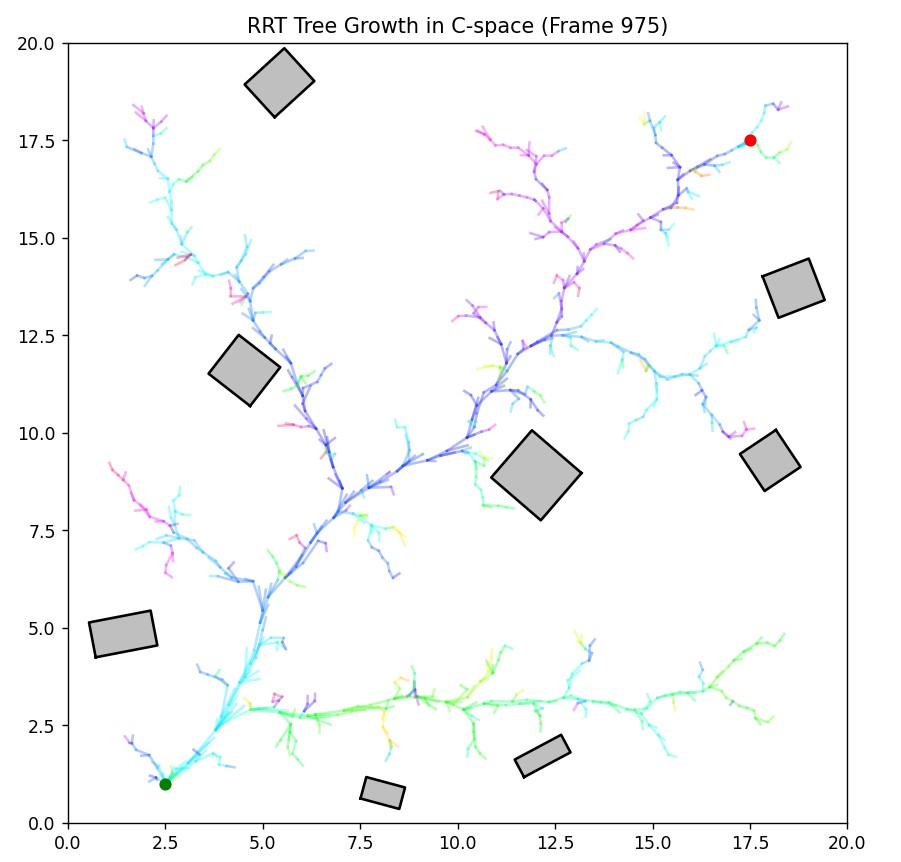
\includegraphics[width=0.5\linewidth]{latex_media/Env3AOTreeGrowthFB1.jpg}
    \caption{Iteration: 1000, Nodes: 975, --robot freeBody --start 2.5 1 0 --goal 17.5 17.5 0 --goal\_rad 0.1 --map Env3.txt}
\end{figure}

\begin{figure} [H]
    \centering
    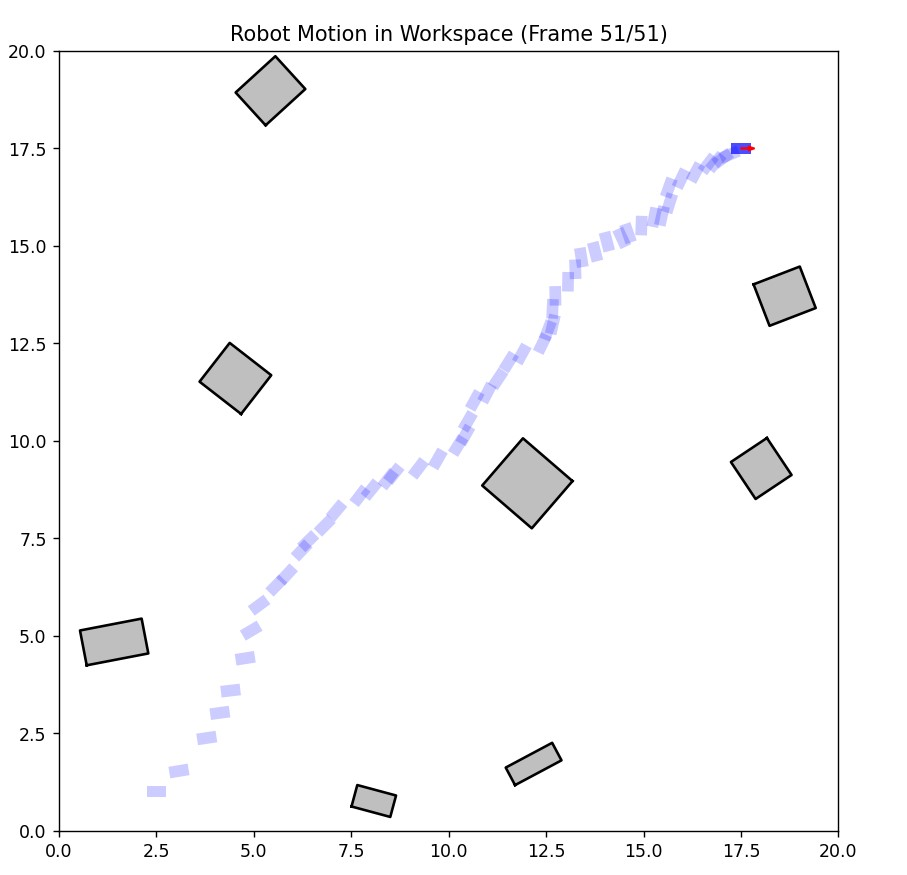
\includegraphics[width=0.5\linewidth]{latex_media/Env3AORobotPathFB1.jpg}
    \caption{Environment 3: FreeBody AO path 1}
\end{figure}

\begin{figure} [H]
    \centering
    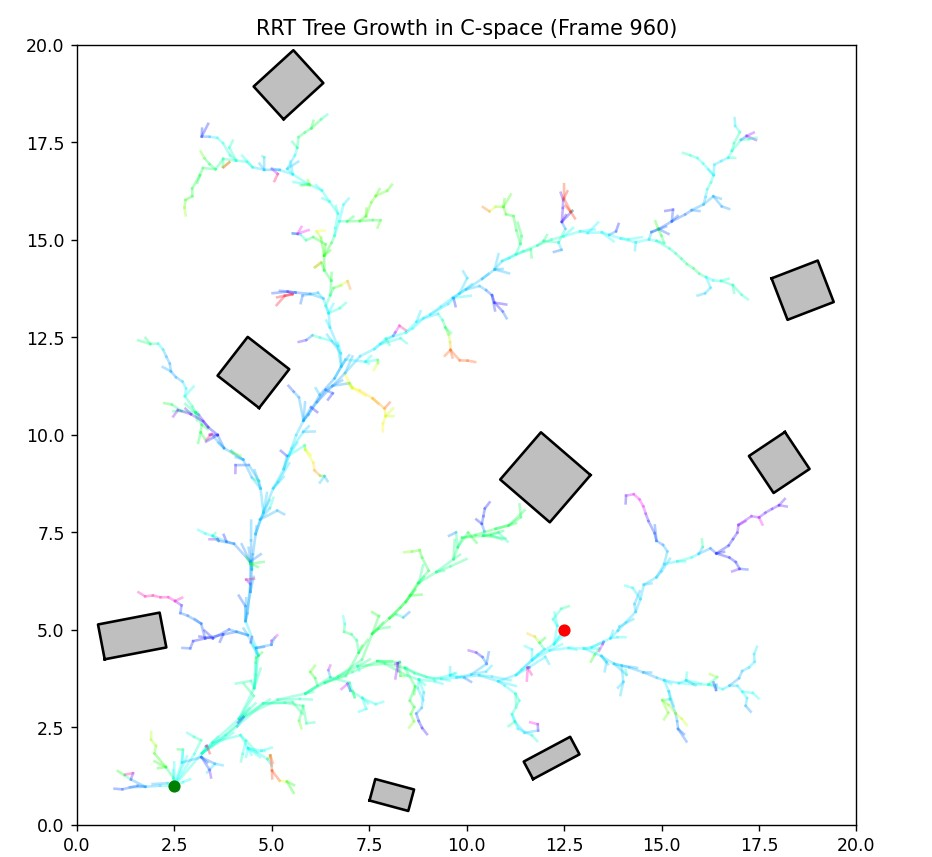
\includegraphics[width=0.5\linewidth]{latex_media/Env3AORobotPathFB2.jpg}
    \caption{Iteration 1000, Nodes: 960, --robot freeBody --start 2.5 1 0 --goal 12.5 5 0 --goal\_rad 0.1 --map Env3.txt}
\end{figure}

\begin{figure} [H]
    \centering
    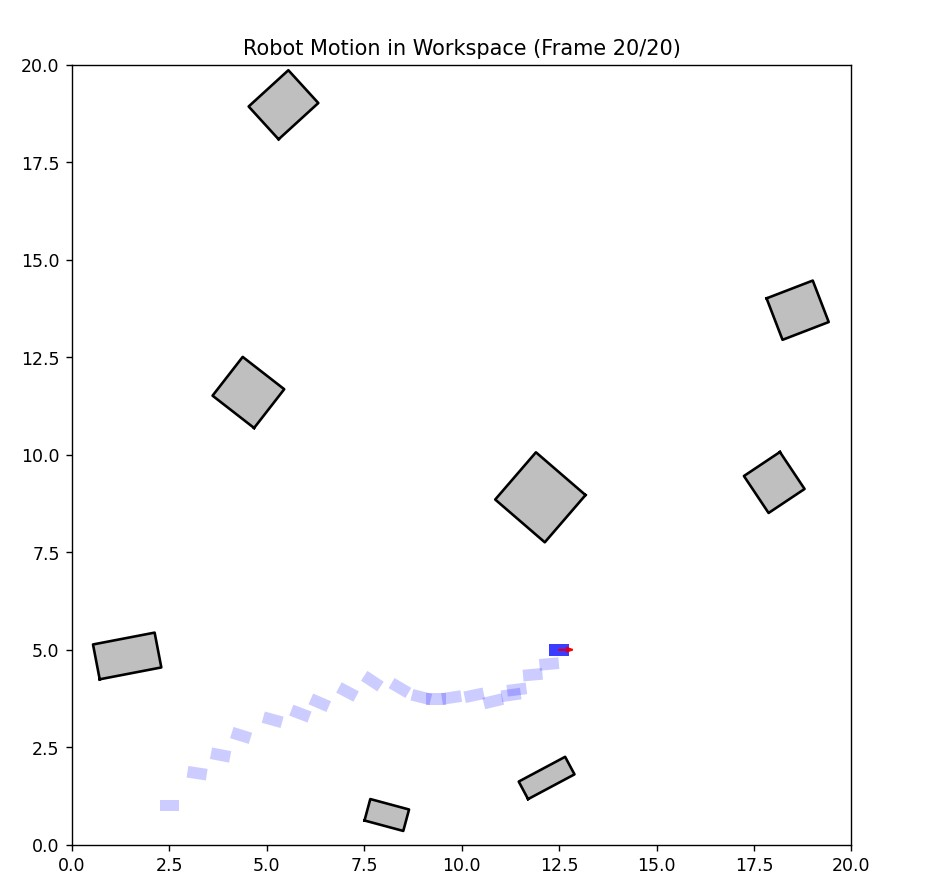
\includegraphics[width=0.5\linewidth]{latex_media/Env3AOTreeGrowthFB2.jpg}
    \caption{Environment 3: FreeBody AO path 2}
\end{figure}

\begin{figure} [H]
    \centering
    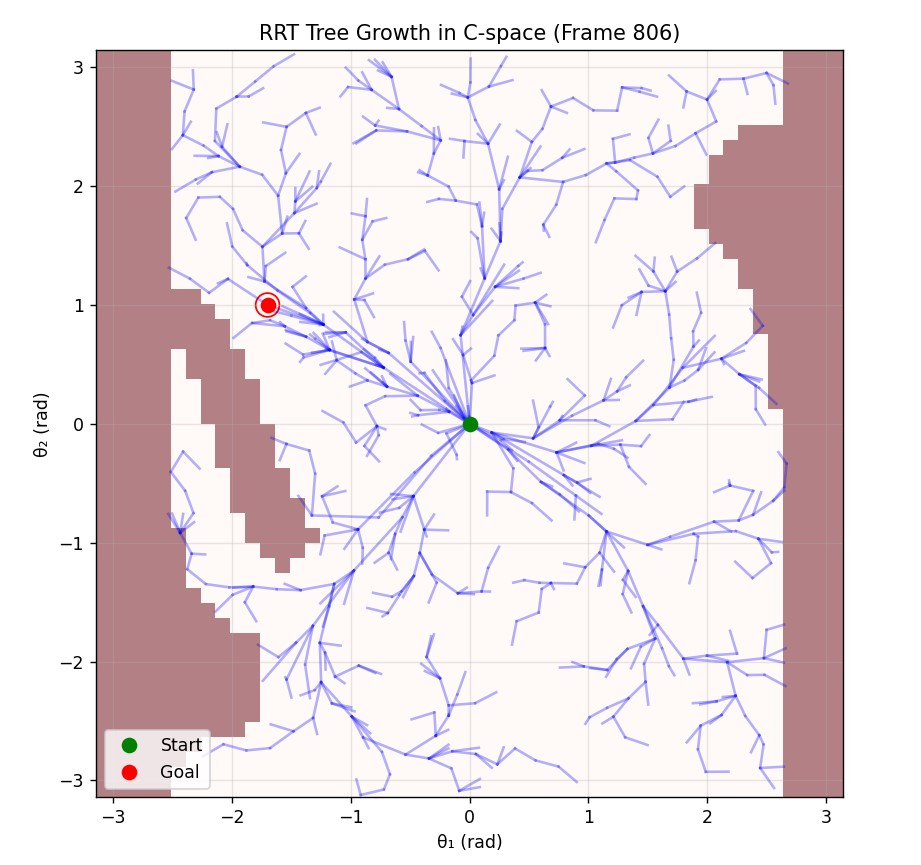
\includegraphics[width=0.5\linewidth]{latex_media/Env4AOTreeGrowthA1.jpg}
    \caption{Iteration: 1000, Nodes: 806, --robot arm --start 0 0 --goal -1.7 1 --goal\_rad 0.1 --map Env4.txt}
\end{figure}

\begin{figure} [H]
    \centering
    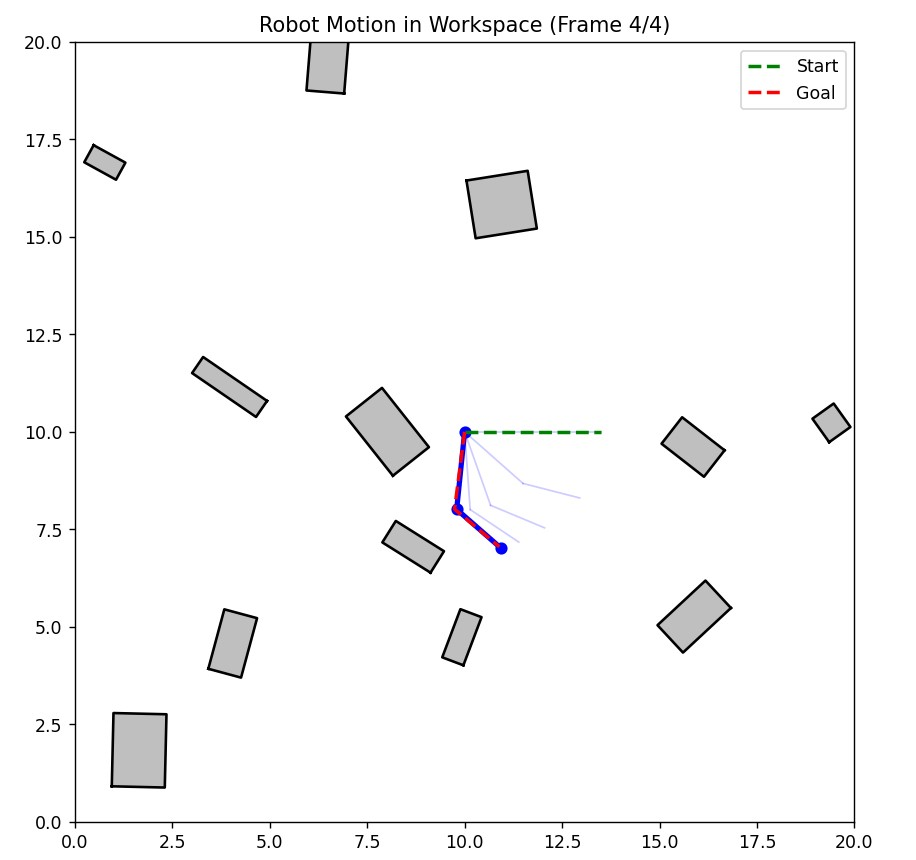
\includegraphics[width=0.5\linewidth]{latex_media/Env4AORobotPathA1.jpg}
    \caption{Environment 4: Arm AO path 1}
\end{figure}

\begin{figure} [H]
    \centering
    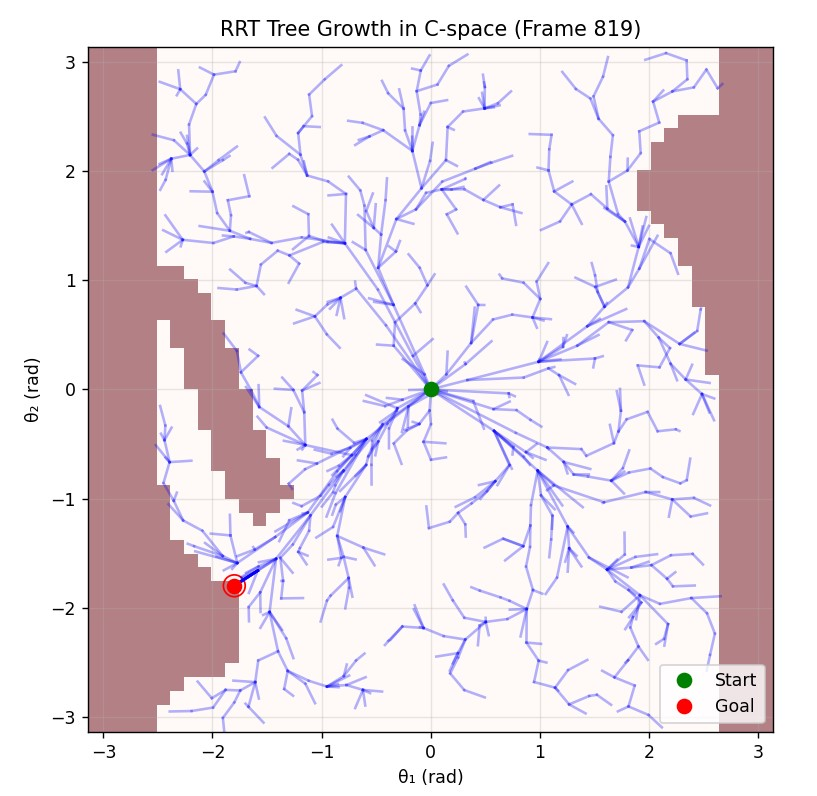
\includegraphics[width=0.5\linewidth]{latex_media/Env4AOTreeGrowthA2.jpg}
    \caption{Iteration: 1000, Nodes: 819, --robot arm --start 0 0 --goal -1.8 -1.8 --goal\_rad 0.1 --map Env4.txt}
\end{figure}

\begin{figure} [H]
    \centering
    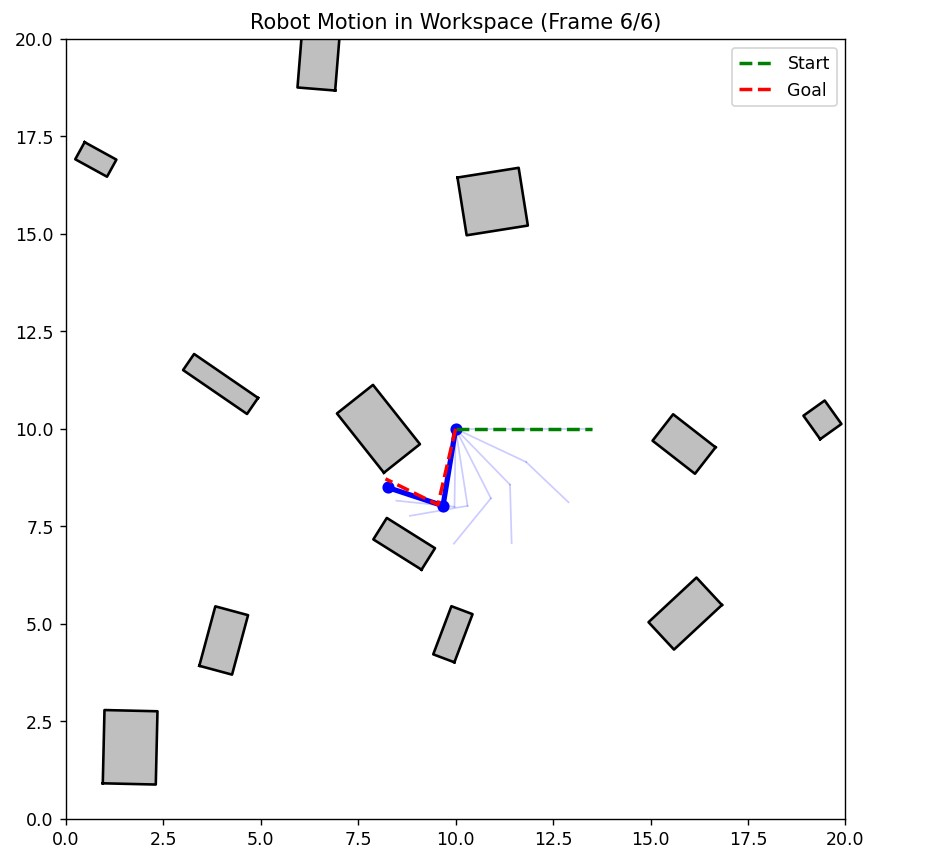
\includegraphics[width=0.5\linewidth]{latex_media/Env4AORobotPathA2.jpg}
    \caption{Environment 4: Arm AO path 2}
\end{figure}

\newpage
\section{Comparison of Planners}
Statistics/Results: \newline
Some context for the results: the trials for each environment were 10 times for each planner, and the results were averaged. The specifications for the trial run are specified for each environment. As you see from the results below, between RRT and the asymptotically optimal RRT*, the paths computed are higher quality in the sense that they are more direct and require fewer nodes since they employ rewiring and costs in the build tree function. The success rate is also slightly higher. The number of iterations and time taken is higher, however, since the algorithm requires more time to be efficient in its nearest neighbor checking, with its dynamic radius in play. You can also see it is especially long for the difficult arm configurations in Environment 4, but it cuts in half the path the RRT version takes. In comparison, PRM performs much faster when planning and determining the best path through the environment. Moreover, the success rate of PRM is 100\% because of the nature of its method of sampling. However, the path that PRM finds is not as high quality compared to that of RRT*. \newline

Env1: (freebody) \newline
--robot freeBody --start 0 0 0 --goal 10 10 0 --goal\_rad 0.1 --map Env1.txt \newline
    PRM:
    \begin{figure} [H]
        \centering
        \includegraphics[width=0.5\linewidth]{latex_media/PRMEnv1Stats.jpg}
        \caption{PRM Environment 1}
    \end{figure}
    RRT: 
    \begin{figure} [H]
        \centering
        \includegraphics[width=0.5\linewidth]{latex_media/RRTEnv1Stats.jpg}
        \caption{RRT Environment 1}
    \end{figure}
    RRT*:
    \begin{figure} [H]
        \centering
        \includegraphics[width=0.5\linewidth]{latex_media/RRTStarEnv1Stats.jpg}
        \caption{RRT* Environment 1}
    \end{figure}

Env2: (arm) \newline
--robot arm --start 0 0 --goal 2 2 --goal\_rad 0.1 --map Env2.txt \newline
    PRM:
    \begin{figure} [H]
        \centering
        \includegraphics[width=0.5\linewidth]{latex_media/PRMEnv2Stats.jpg}
        \caption{PRM Environment 2}
    \end{figure}
    RRT: 
    \begin{figure} [H]
        \centering
        \includegraphics[width=0.5\linewidth]{latex_media/RRTEnv2Stats.jpg}
        \caption{RRT Environment 2}
    \end{figure}
    RRT*: 
    \begin{figure} [H]
        \centering
        \includegraphics[width=0.5\linewidth]{latex_media/RRTStarEnv2Stats.jpg}
        \caption{RRT* Environment 2}
    \end{figure}

Env3: (freebody) \newline
--robot freeBody --start 2.5 2.5  0 --goal 2.5 15 0 --goal\_rad 0.1 --map Env3.txt \newline
    PRM:
    \begin{figure} [H]
        \centering
        \includegraphics[width=0.5\linewidth]{latex_media/PRMEnv3Stats.jpg}
        \caption{PRM Environment 3}
    \end{figure}
    RRT: 
    \begin{figure} [H]
        \centering
        \includegraphics[width=0.5\linewidth]{latex_media/RRTEnv3Stats.jpg}
        \caption{RRT Environment 3}
    \end{figure}
    
    RRT*: 
    \begin{figure} [H]
        \centering
        \includegraphics[width=0.5\linewidth]{latex_media/RRTStarEnv3Stats.jpg}
        \caption{RRT* Environment 3}
    \end{figure}

Env4: (arm) \newline
--robot arm --start 0 0 --goal -1.7 -1.5 --goal\_rad 0.1 --map Env4.txt \newline
    PRM:
    \begin{figure} [H]
        \centering
        \includegraphics[width=0.5\linewidth]{latex_media/PRMEnv4Stats.jpg}
        \caption{PRM Environment 4}
    \end{figure}
    RRT: 
    \begin{figure} [H]
        \centering
        \includegraphics[width=0.5\linewidth]{latex_media/RRTEnv4Stats.jpg}
        \caption{RRT Environment 4}
    \end{figure}
    
    RRT*: 
    \begin{figure} [H]
        \centering
        \includegraphics[width=0.5\linewidth]{latex_media/RRTStarEnv4Stats.jpg}
        \caption{RRT* Environment 4}
    \end{figure}

Env5: (freebody) \newline
--robot freeBody --start 2.5 1 0 --goal 15 16.1 0 --goal\_rad 0.1 --map Env5.txt \newline
    PRM:
    \begin{figure} [H]
        \centering
        \includegraphics[width=0.5\linewidth]{latex_media/PRMEnv5Stats.jpg}
        \caption{PRM Environment 5}
    \end{figure}
    RRT: 
    \begin{figure} [H]
        \centering
        \includegraphics[width=0.5\linewidth]{latex_media/RRTEnv5Stats.jpg}
        \caption{RRT Environment 5}
    \end{figure}
    
    RRT*: 
    \begin{figure} [H]
        \centering
        \includegraphics[width=0.5\linewidth]{latex_media/RRTStarEnv5Stats.jpg}
        \caption{RRT* Environment 5}
    \end{figure}

\section{Motion Planning for a Car-like Mobile Robot}
There are a lot of differences when dealing with a non-holonomic robot in the case of a car. Since we have to deal with many movement constraints, the RRT planner becomes less effective when finding a feasible path. It can find paths to get to the goal like the free body, but it's harder for it to allow the car to move that way. For the goal checking, in addition to the distance checking the heading angle and steering angle had to be checked for it to be achievable. Specifically for car parameters, we kept the length and width but added a max steering angle and velocity since it can't just translate to the next node. Since it was no longer a straight edge leading to the next configuration we kept track of these in our trajectory array. We applied kinematic equations with the velocity and time moving to update the x, y, and theta of the current configuration that would extend to the new node we found when building our tree. This simulation of the car motion would give us a trajectory of configurations to follow to connect the nodes. Since we have a trajectory of configurations, we would have to check for collisions for all of them. Another update is the random configuration now also includes the steering angle. The steer function is also updated to calculate the appropriate steer angle and simulate the car's motion. When checking the goal, the steering angle is also adjusted. You will see when building the tree, it seems like the robot reached the goal configuration but continues to search, most likely because the path wasn't feasible for a non-holonomic robot. 

Below you will see plots for the 5 environments we ran the tests on. You can see in the visualizations how the car is actually moving, and that it needs to steer and turn to reach its goal. Even in the tree growth, you can see there are multiple paths that seem to reach the goal, but they are probably not feasible for a car robot to take if the steering is too sharp. In the last environment, you can even see it take a loop to adjust for the steering.  

(Note the labels are the same as the environments above, they are supposed to be x and y for the plots) (Same naming convention as before where "Env1car\_rrt\_grow" would mean the tree growth for car RRT algorithm ran on environment 1, traj is for the solution path )

\begin{figure} [H]
    \centering
    \includegraphics[width=0.5\linewidth]{latex_media/Env1Car_rrt_grow.jpg}
    \caption{Iteration: 205, Nodes: 183, --robot car --start 0 0 0 0 --goal 10 10 0 0 --goal\_rad 0.5 --map Env1.txt}
\end{figure}

\begin{figure} [H]
    \centering
    \includegraphics[width=0.5\linewidth]{latex_media/Env1Car_rrt_traj.jpg}
    \caption{Environment 1: RRT Car Traj}
\end{figure}

\begin{figure} [H]
    \centering
    \includegraphics[width=0.5\linewidth]{latex_media/Env2Car_rrt_grow.jpg}
    \caption{Iteration: 710, Nodes: 611, --robot car --start 0 0 0 0 --goal 15 10 0 0 --goal\_rad 0.5 --map Env2.txt}
\end{figure}

\begin{figure} [H]
    \centering
    \includegraphics[width=0.5\linewidth]{latex_media/Env2Car_rrt_traj.jpg}
    \caption{Environment 2: RRT Car Traj}
\end{figure}

\begin{figure} [H]
    \centering
    \includegraphics[width=0.5\linewidth]{latex_media/Env3Car_rrt_grow.jpg}
    \caption{Iteration: 307, Nodes: 257, --robot car --start 2.5 2.5 0 0 --goal 15 15 0 0 --goal\_rad 0.5 --map Env3.txt}
\end{figure}

\begin{figure} [H]
    \centering
    \includegraphics[width=0.5\linewidth]{latex_media/Env3Car_rrt_traj.jpg}
    \caption{Environment 3: RRT Car Traj}
\end{figure}

\begin{figure} [H]
    \centering
    \includegraphics[width=0.5\linewidth]{latex_media/Env4Car_rrt_grow.jpg}
    \caption{Iteration: 887, Nodes: 729,  --robot car --start 5 1 0 0 --goal 15 15 0 0 --goal\_rad 0.5 --map Env4.txt}
\end{figure}

\begin{figure} [H]
    \centering
    \includegraphics[width=0.5\linewidth]{latex_media/Env4Car_rrt_traj.jpg}
    \caption{Environment 4: RRT Car Traj}
\end{figure}

\begin{figure} [H]
    \centering
    \includegraphics[width=0.5\linewidth]{latex_media/Env5Car_rrt_grow.jpg}
    \caption{Iteration: 959, Nodes: 621, --robot car --start 2.5 1 0 0 --goal 15 13 0 0 --goal\_rad 0.5 --map Env5.txt}
\end{figure}

\begin{figure} [H]
    \centering
    \includegraphics[width=0.5\linewidth]{latex_media/Env5Car_rrt_traj.jpg}
    \caption{Environment 5: RRT Car Traj}
\end{figure}

\end{document}